% !TEX root = ../thesis-WW.tex

\chapter{Bayesian Attitude and Position Estimation with Matrix Fisher-Gaussian Distribution} \label{chap:pose-estimation}

In the previous chapter, the MFG is applied in the classic attitude estimation problem, where it is demonstrated through simulation that the filter designed using MFG has better accuracy than MEKF in challenging cases when the attitude has large uncertainty.
In inertial navigation, the estimated attitude is used to transform the linear acceleration measured by an accelerometer into the inertial frame, which can be integrated twice into position after the gravity component is subtracted.
In this chapter, the filter for attitude estimation is generalized into this inertial navigation setting using MFG.
In particular, the linear part of MFG is augmented into $\mathbb{R}^{12}$, including the linear velocity, position, gyroscope and accelerometer biases.

In Chapter \ref{section:posEst}, the position measurement given by a GNSS receiver is considered in the measurement update step.
Then in Chapter \ref{section:VIO}, it is replaced by camera measurements of the locations for unknown features or known landmarks.
It is assumed that the camera is an RGB-D or stereo camera, so that projection measurements have already been triangulated into 3D locations.
These filters are compared with variants of MEKF \cite{sola2017quaternion} through simulation studies, where it is shown that the filters based on MFG have faster convergence rate when the initial heading direction is completely unknown, which is frequently encountered in practical localization problems.

\section{Loosely Coupled IMU-GNSS Integration} \label{section:posEst}

In this section, the attitude estimation problem considered in Chapter \ref{section:attEst} is extended into a full inertial navigation problem.
More specifically, it is assumed that an inertial measurement unit (IMU) is attached to a rigid body, which has a gyroscope measuring the angular velocity, and an accelerometer measuring the linear acceleration, both in the body fixed frame.
The linear acceleration can be transformed into the inertial frame using the integrated attitude, and then it can be integrated twice into position after subtracting the gravity component.
It is also assumed that a global navigation satellite system (GNSS) receiver provides position measurements of the rigid body, which are used to correct the attitude and position integrated using the IMU.
Since the pseudorange from GNSS is first converted into position measurements, and then used to correct the inertial navigation estimation, this is usually referred to as loosely coupled IMU-GNSS integration.

The MEKF for attitude estimation can be generalized to deal with this inertial navigation setting \cite{sola2017quaternion}.
However, as discussed in previous sections, it cannot handle large attitude uncertainty due to its inherent Gaussian assumption.
Similar as in attitude estimation, the MFG is used to design a new estimator, which is suitable for large attitude uncertainty.
This is particularly advantageous in some practical problems, for example, when the IMU starts in a building, where the heading direction is usually completely unknown; or when the GNSS receiver cannot receive signal for a long period time, and the uncertainty for inertial navigation accumulates.

The definition of MFG is flexible enough to handle this inertial navigation setting, as its linear part can be arbitrary in $\mathbb{R}^n$.
This makes MFG distinguished from the distribution defined for dual quaternions \cite{li2019geometry,li2020unscented}, where the linear part must be position only.
In this section, the MFG is used to design a Bayesian filter that estimates attitude, gyroscope bias, position, linear velocity, and accelerometer bias concurrently.

\subsection{Problem Formulation}

The IMU kinematic model is formulated in discrete time as follows.
\begin{align}
	R_{k+1} &= R_k \expb{ h(\hat{\Omega}_k + \hat{b}_{g,k}) + H_{gu}\Delta W_{gu} }, \label{eqn:posEst-kinematics-attitude} \\
	b_{g,k+1} &= b_{g,k} + H_{gv}\Delta W_{gv}, \label{eqn:posEst-kinematics-gyrobias} \\
	p_{k+1} &= p_k + hv_k, \label{eqn:posEst-kinematics-pos} \\
	v_{k+1} &= v_k - gh + R_k\left( h(a_k+b_{a,k}) + H_{au}\Delta W_{au} \right), \label{eqn:posEst-kinematics-velocity} \\
	b_{a,k+1} &= b_{a,k} + H_{av}\Delta W_{av}, \label{eqn:posEst-kinematics-accebias}
\end{align}
where $R\in\SO{3}$ is the attitude, $x = \big[b_g^T, p^T, v^T, b_a^T\big]^T \in \mathbb{R}^{12}$ are gyroscope bias, position, linear velocity and accelerometer bias, respectively.
The position and linear velocity are resolved in the inertial frame.
The gravity vector in the inertial frame is denoted by $g\in\mathbb{R}^3$.
Next, $\Omega\in\mathbb{R}^3$ is the angular velocity measured by the gyroscope, and $a\in\mathbb{R}^3$ is the linear acceleration measured by the accelerometer, and they are resolved in the body-fixed frame.
The angular velocity measurement is affected by two noises: $H_{gu}\Delta W_{gu}$ is a white noise, and $b_g$ is a random walk bias driven by $H_{gv}\Delta W_{gv}$.
The noises for accelerometer are similar, given by the white noise $H_{au}\Delta W_{au}$, and the bias driven by $H_{av}\Delta W_{av}$.
These noise terms are Gaussian with
\begin{align}
	&H_{gu}\Delta W_{gu} \sim \mathcal{N}(0,hG_{gu}), \quad H_{gv}\Delta W_{gv} \sim \mathcal{N}(0,hG_{gv}), \label{eqn:posEst-gyroNoise} \\
	&H_{au}\Delta W_{au} \sim \mathcal{N}(0,hG_{au}), \quad H_{av}\Delta W_{av} \sim \mathcal{N}(0,hG_{av}),
\end{align}
where $G_{gu} = H_{gu}H_{gu}^T$, $G_{gv} = H_{gv}H_{gv}^T$, $G_{au} = H_{au}H_{au}^T$, $G_{av} = H_{av}H_{av}^T$, and they are independent.
Finally, the subscript $k$ denote the time step, and $h = t_{k+1}-t_k$ is the constant sampling period for any $k$.

It is assumed that the position $p_k$ is measured by a GNSS receiver at time $t_k$, denote by $y_k\in\mathbb{R}^3$.
The measurement noise is Gaussian, i.e.,
\begin{align}
	y_k|p_k = p_k + \mathcal{N}(0,\Sigma_y).
\end{align}
Optionally, the attitude and some reference directions can also be measured as formulated in Chapter \ref{section:attEst-problem}.
Namely, the attitude can be directly measured by $N_a$ sensors as $Z_i$, and the measurement noises follow matrix Fisher distributions with parameters $F_{Z_i}$, for $i=1,\ldots,N_a$.
Also, $N_v$ fixed reference directions $a_j\in\Sph^2$ in inertial frame are measured as $z_j\in\Sph^2$ in the body-fixed frame, and the measurement noises follow von Mises-Fisher distribution with the mean direction $R_t^TB_ja_j$, and concentration parameter $\kappa$, where $R_t\in\SO{3}$ is the true attitude, for $j = 1,\ldots,N_v$.
All measurements at time $t_k$ are denoted by $\mathcal{Z}_k$.

Suppose $(R_0,x_0) = (R_0,b_{g,0},p_0,v_0,b_{a,0})$ at the initial time $t_0$ follow an MFG with $n=12$ and parameters $(\mu_0,\Sigma_0,P_0,U_0,S_0,V_0)$ of appropriate dimensions.
Given the IMU measurements $\{\Omega_k,a_k\}_{k=1}^\infty$, and all position, attitude, and direction measurements $\mathcal{Z}_{k=1}^\infty$, the problem is to find the posterior distribution of $(R_k,x_k) | \{\mathcal{Z}_m\}_{m=1}^k$, and approximate it to an MFG with parameters $(\mu_k, \Sigma_k, P_k, U_k, S_k, V_k)$.
Similar to the attitude estimator, two steps are needed.
In the uncertainty propagation step, the posterior distribution $(R_k,x_k) | \{\mathcal{Z}_m\}_{m=1}^k$ is propagated using the IMU kinematic equations \eqref{eqn:posEst-kinematics-attitude}-\eqref{eqn:posEst-kinematics-accebias} to the next time step as $(R_{k+1},x_{k+1}) | \{\mathcal{Z}_m\}_{m=1}^k$.
Next, the propagated distribution is updated by the measurements $\mathcal{Z}_{k+1}$ using Bayes' formula into $(R_{k+1},x_{k+1}) | \{\mathcal{Z}_m\}_{m=1}^{k+1}$.
In the next two subsections, algorithms for these two steps are developed.

\subsection{Uncertainty Propagation} \label{section:posEst-propagation}

Suppose $(R_k,x_k) | \{\mathcal{Z}_m\}_{m=1}^k \sim \mathcal{MG}(\mu_k, \Sigma_k, P_k, U_k, S_k, V_k)$.
In this subsection, the moments of $(R_{k+1},x_{k+1})$ required for the MLE of MFG are calculated using the IMU kinematics equations \eqref{eqn:posEst-kinematics-attitude}-\eqref{eqn:posEst-kinematics-accebias}.
One way of calculating those moments is to propagated deterministically sampled sigma points through the kinematic equations using the unscented transform of MFG, as introduced in Chapter \ref{section:attEst-propagation}.
This approach can be easily generalized to the inertial navigation settings considered in this subsection, and will not be discussed here.
Instead, this subsection calculates approximate analytical expressions of the required moments.

First, because \eqref{eqn:posEst-kinematics-attitude} and \eqref{eqn:posEst-kinematics-gyrobias} are exactly the same as the attitude kinematics considered in \eqref{eqn:attEst-kinematics-att-dist} and \eqref{eqn:attEst-kinematics-bias-dist}, the moment $\expect{R_{k+1}}$ can be calculated using Theorem \ref{thm:attEst-prop-E(R_{k+1})}.
Then $\expect{R_{k+1}}$ is used in the marginal MLE of MFG to obtain the parameters $U_{k+1}$, $S_{k+1}$, and $V_{k+1}$.
Next, define $Q_{k+1} = U_{k+1}^TR_{k+1}V_{k+1}$, and $\nu_{R_{k+1}} = (Q_{k+1}S_{k+1}-S_{k+1}Q_{k+1}^T)^\vee$ for MFGI, or $\nu_{R_{k+1}} = (S_{k+1}Q_{k+1}-Q_{k+1}^TS_{k+1})^\vee$ for MFGB as the intermediate parameters for the MFG at time $t_{k+1}$.
According to Theorem \ref{thm:MFG-MLE-conditional}, $\expect{x_{k+1}}$, $\expect{x_{k+1}\nu_{R_{k+1}}^T}$, $\expect{x_{k+1}x_{k+1}^T}$, and $\expect{\nu_{R_{k+1}}\nu_{R_{k+1}}^T}$ need to be calculated.
Note that $\expect{\nu_{R_{k+1}}\nu_{R_{k+1}}^T}$ is only involved with the gyroscope kinematics \eqref{eqn:posEst-kinematics-attitude} and \eqref{eqn:posEst-kinematics-gyrobias}, so it can be calculated using \eqref{eqn:attEst-prop-EvRvR_{k+1}} in Theorem \ref{thm:attEst-prop-otherMoments}.
In the remainder of this subsection, the calculations for $\expect{x_{k+1}}$, $\expect{x_{k+1}\nu_{R_{k+1}}^T}$, and $\expect{x_{k+1}x_{k+1}^T}$ are developed.

In perpetration for these calculations, the parameters $\mu_k$, $P_k$ and $\Sigma_k$ are written for each component in block form as
\begin{gather} \label{eqn:posEst-prop-blocks}
	\allowdisplaybreaks
	\mu_k = \begin{bmatrix}
		\mu_{b_g,k} \\ \mu_{p,k} \\ \mu_{v,k} \\ \mu_{b_a,k}
	\end{bmatrix}, \qquad
	P_k = \begin{bmatrix}
		P_{b_g,k} \\ P_{p,k} \\ P_{v,k} \\ P_{b_a,k}
	\end{bmatrix}, \qquad
	\Sigma_k = \begin{bmatrix}
		\Sigma_{b_gb_g,k} & \Sigma_{b_gp,k} & \Sigma_{b_gv,k} & \Sigma_{b_gb_a,k} \\
		\Sigma_{pb_g,k} & \Sigma_{pp,k} & \Sigma_{pv,k} & \Sigma_{pb_a,k} \\
		\Sigma_{vb_g,k} & \Sigma_{vp,k} & \Sigma_{vv,k} & \Sigma_{vb_a,k} \\
		\Sigma_{b_ab_g,k} & \Sigma_{b_ap,k} & \Sigma_{b_av,k} & \Sigma_{b_ab_a,k}
	\end{bmatrix}.
\end{gather}
With these, the calculation for $\expect{x_{k+1}}$ is presented in the next theorem.

\begin{theorem} \label{thm:posEst-prop-Ex}
	The moment $\expect{x_{k+1}} = \expect{ b_{g,k+1}^T, p_{k+1}^T, v_{k+1}^T, b_{a,k+1}^T}^T$ are given by
	\begin{align}
		\expect{b_{g,k+1}} &= \expect{b_{g,k}} \\
		\expect{p_{k+1}} &= \expect{p_k} + h\expect{v_k} \\
		\expect{v_{k+1}} &= \expect{v_k} + h\expect{R_k}(a_k+\mu_{b_a,k}) + h\expect{R_kP_{b_a,k}\nu_{R_k}} - gh, \\
		\expect{b_{a,k+1}} &= \expect{b_{a,k}}
	\end{align}
	where $\nu_{R_k} = (Q_kS_k-S_kQ_k^T)^\vee$ for MFGI, or $\nu_{R_k} = (S_kQ_k-Q_k^TS_k)^\vee$ for MFGB, with $Q_k = U_k^TR_kU_k$.
\end{theorem}
\begin{proof}
	The first, second, and fourth equations are immediate from \eqref{eqn:posEst-kinematics-gyrobias}, \eqref{eqn:posEst-kinematics-pos}, and \eqref{eqn:posEst-kinematics-accebias}, because $\Delta W_{gv}$ and $\Delta W_{av}$ have zeros means.
	For the third equation, a similar calculation as \eqref{eqn:MFG-Exx-proof} shows that
	\begin{align*}
		\expect{R_kb_{a,k}} = \expect{R_k}\mu_{b_a,k} + \expect{R_kP_{b_a,k}\nu_{R_k}},
	\end{align*}
	and the desired result is proved.
\end{proof}

The expressions for $\expect{x_{k+1}\nu_{R_{k+1}}^T}$ and $\expect{x_{k+1}x_{k+1}^T}$ are very tedious, and they are relegated to Appendix \ref{app:posEst-prop-moments}.
Note that these two moments, $\expect{\nu_{R_{k+1}}\nu_{R_{k+1}}^T}$, and $\expect{x_{k+1}}$ can be calculated using up to the third order moments of $Q_k\sim\mathcal{M}(S_k)$, with the accuracy of $O(h^2)$.
Then using Theorem \ref{thm:MFG-MLE-conditional}, the parameters $\mu_{k+1}$, $P_{k+1}$ and $\Sigma_{k+1}$ can be obtained.
In summary, the uncertainty $S(R_k,x_k) \sim \mathcal{MG}(\mu_k, \Sigma_k, P_k, U_k, S_k, V_k)$ at time $t_k$ is propagated into $(R_{k+1},x_{k+1}) \sim \mathcal{MG}(\mu_{k+1},\allowbreak \Sigma_{k+1},\allowbreak P_{k+1},\allowbreak U_{k+1},\allowbreak S_{k+1},\allowbreak V_{k+1})$, up to accuracy $O(h^2)$ in moments.
The pseudocode for this uncertainty propagation scheme is summarized in Table \ref{tab:posEst-prop}.

\begin{table}
	\caption{Uncertainty propagation for IMU kinematics}
	\label{tab:posEst-prop}
	\begin{algorithmic}[1]
		\algrule[0.8pt]
		\Procedure{$\mathcal{MG}(t_{k+1}) = $ Uncertainty Propagation}{$\mathcal{MG}(t_k),\Omega_k,a_k$}
		\algrule
		\State Calculate $\expect{R_{k+1}}$ using \eqref{eqn:attEst-prop-E(R_{k+1})} with $\mu_k$, $P_k$, $G_u$ replaced by $\mu_{b_g,k}$, $P_{b_g,k}$ in \eqref{eqn:posEst-prop-blocks}, and $G_{gu}$ in \eqref{eqn:posEst-gyroNoise}, respectively.
		\State Obtain $U_{k+1},S_{k+1},V_{k+1}$ according to Chapter \ref{section:MFG-property} using $\expect{R_{k+1}}$.
		\State Calculate $\expect{\nu_{R_{k+1}}\nu_{R_{k+1}}^T}$ using \eqref{eqn:attEst-prop-EvRvR_{k+1}}, calculate $\expect{x_{k+1}}$, $\expect{x_{k+1}\nu_{R_{k+1}}^T}$ and $\expect{x_{k+1}x_{k+1}^T}$ with Theorem \ref{thm:posEst-prop-Ex}, Theorem \ref{thm:posEst-prop-ExvR}, and Theorem \ref{thm:posEst-prop-Exx}, respectively.
		\State Obtain $\mu_{k+1},\Sigma_{k+1},P_{k+1}$ according to Theorem \ref{thm:MFG-MLE-conditional} using the moments calculated in Step 4.
		\State Set $\mathcal{MG}(t_{k+1}) = \mathcal{MG}(\mu_{k+1},\Sigma_{k+1},P_{k+1},U_{k+1},S_{k+1},V_{k+1})$.
		\EndProcedure
		\algrule[0.8pt]
	\end{algorithmic}
\end{table}

\subsection{Measurement Update} \label{section:posEst-update}

The algorithm for propagating the posterior distribution $(R_k,x_k) | \{\mathcal{Z}_{m}\}_{m=1}^k$ at time $t_k$ into the prior distribution $(R_{k+1},x_{k+1}) | \{\mathcal{Z}_{m}\}_{m=1}^k$ at time $t_{k+1}$ has been introduced in the previous subsection.
In this subsection, the prior distribution $(R_{k+1},x_{k+1}) | \{\mathcal{Z}_{m}\}_{m=1}^k$ is updated into the posterior distribution $(R_{k+1},x_{k+1}) | \{\mathcal{Z}_{m}\}_{m=1}^{k+1}$ at time $t_{k+1}$, with the measurements $\mathcal{Z}_{k+1}$ using Bayes' formula.
Since the update is completed instantaneously at time $t_{k+1}$, the subscript $k+1$ is omitted in this subsection, and the variables relevant to the posterior distribution are denoted by the superscript $+$.

Suppose the prior distribution of $(R,x)$ before measurement update follows MFG with parameters $(\mu,\Sigma,P,U,S,V)$. 
By the Bayes' rule and Theorem 3.2 in \cite{lee2018bayesian}, the posterior density conditioned on all of the available measurements $\mathcal{Z}$ is 
\begin{align} \label{eqn:posEst-update-density}
	&p(R,x\lvert \mathcal{Z}) \propto \etr{ \bigg( F + \sum_{i=1}^{N_a}Z_iF_i^T + \sum_{j=1}^{N_v}\kappa_jB_ja_jz_j^T \bigg)R^T } \nonumber \\
	&\quad \cdot \expb{-\tfrac{1}{2}(x-\mu_c)^T\Sigma_c^{-1}(x-\mu_c)} \cdot \expb{-\tfrac{1}{2}(Hx-y)^T\Sigma_y^{-1}(Hx-y)},
\end{align}
where $H = [0_{3\times 3}, I_{3\times 3}, 0_{3\times 6}]$ selects the position component from $x$, and $F$, $\mu_c$ and $\Sigma_c$ are defined as in Definition \ref{def:MFG} with respect to $\mathcal{MG}(\mu,\Sigma,P,U,S,V)$.
Compared with \eqref{eqn:attEst-update-density} in attitude estimation, \eqref{eqn:posEst-update-density} has an additional term contributed by the position measurement coming from the GNSS receiver.

To deal with this posterior density, it is first shown that \eqref{eqn:posEst-update-density} can be factorized into the marginal component for $R$, and the conditional component for $x|R$.
\begin{lemma} \label{lemma:posEst-update-factor}
	Let $\tilde{F}$ be defined as the $F^+$ in \eqref{eqn:attEst-update-F}, or $\tilde{F} = F$ if there are no attitude or direction measurements.
	Also, define the ``Kalman gain''
	\begin{align}
		K = \Sigma_cH^T(H\Sigma_cH^T + \Sigma_y)^{-1} \in \mathbb{R}^{12\times 3}.
	\end{align}
	Then the posterior density \eqref{eqn:posEst-update-density} can be factorized into two parts:
	\begin{align} \label{eqn:posEst-update-density-factor}
		p(R,x|\mathcal{Z}) = f_R(R) f_{x|R}(x|R),
	\end{align}
	where the marginal part $f_R(R)$ is given by
	\begin{align} \label{eqn:posEst-update-density-R}
		f_R(R) \propto \etr{\tilde{F}R^T} \expb{-\tfrac{1}{2}(H\mu_c-y)^T (\Sigma_y+H\Sigma_cH^T)^{-1} (H\mu_c-y)},
	\end{align}
	and the conditional part $f(x|R)$ is given by
	\begin{align} \label{eqn:posEst-update-density-x|R}
		f_{x|R}(x|R) \propto \expb{-\tfrac{1}{2} \big(x-(I-KH)\mu_c-Ky\big)^T \big((I-KH)\Sigma_c\big)^{-1} \big(x-(I-KH)\mu_c-Ky\big)},
	\end{align}
	where $I$ is an abbreviation of $I_{12\times 12}$.
\end{lemma}
\begin{proof}
	Using a similar technique that is used to prove the linear Kalman filter, and the Woodbury matrix identity \cite{petersen2008matrix}, it can be shown that
	\begin{align*}
		&\expb{-\tfrac{1}{2}(x-\mu_c)^T\Sigma_c^{-1}(x-\mu_c)} \cdot \expb{-\tfrac{1}{2}(Hx-y)^T\Sigma_y^{-1}(Hx-y)} \\
		= &\expb{-\tfrac{1}{2} \big(x-(I-KH)\mu_c-Ky\big)^T \big((I-KH)\Sigma_c\big)^{-1} \big(x-(I-KH)\mu_c-Ky\big)} \\
		&\qquad \cdot \expb{-\tfrac{1}{2}(H\mu_c-y)^T (\Sigma_y+H\Sigma_cH^T)^{-1} (H\mu_c-y)},
	\end{align*}
	which gives the desired \eqref{eqn:posEst-update-density-factor}.
\end{proof}

Note that the marginal part $f_R(R)$ does not depend on $x$, so according to the marginal-conditional MLE of MFG, the first step is to approximate $f_R(R)$ into the density function of a matrix Fisher distribution.
Since the $\mu_c$ is linear in $R$, $f_R(R)$ has quadratic terms of $R$ in its exponent, making the expectation $\expect{R}$ corresponding to $f_R(R)$ impractical to be calculated directly from the density function.
Instead, $\expect{R}$ is approximated using the unscented transform of matrix Fisher distribution \cite{gilitschenski2015unscented,lee2018bayesian} \footnote{The unscented transform in \cite{gilitschenski2015unscented} is developed for the Bingham distribution, and it can be converted to the matrix Fisher distribution using Theorem \ref{thm:Bh2MF}}.
The idea is that the weighted sigma points $\{R_i,w_i\}_{i=1}^7$ are selected from $\mathcal{M}(\tilde{F})$, corresponding to the first part of \eqref{eqn:posEst-update-density-R}.
The weights are reweighed by the second part of \eqref{eqn:posEst-update-density-R} as
\begin{align} \label{eqn:posEst-update-sigmapoints}
	w_i^+ = w_i \expb{-\tfrac{1}{2}(H\mu_{c,i}-y)^T (\Sigma_y+H\Sigma_cH^T)^{-1} (H\mu_{c,i}-y)},
\end{align}
where $\mu_{c,i}$ are calculated using $R_i$ as in \eqref{eqn:MFG-Miuc}, for $i=1,\dots,7$.
Then the moment $\expect{R}$ is approximated using these reweighed sigma points as $\sum_{i=1}^7 w_i^+R_i$ after normalization.
This update procedure comes from particle filters \cite{arulampalam2002tutorial} where the deterministic sigma points are replaced by the randomly sampled particles, and has been widely applied in Bayesian filters with nonlinear measurement functions \cite{kurz2016recursive}.

However, as noted in \cite{kurz2016recursive}, the approximation of $\expect{R}$ using this technique can sometimes degenerate, i.e., some or all of $w_i^+$ can be close to zero due to large discrepancies between $H\mu_{c,i}$ and $y$.
To overcome this problem, the ``progressive update'' developed in \cite{hanebeck2013pgf} is used here, which has been applied to several stochastic filters \cite{huang2015gaussian,kurz2014nonlinear,li2021progressive}.
Denote the second term on the right hand side of \eqref{eqn:posEst-update-density-R} as $f_m(R)$.
The idea of progressive update is that instead of multiplying the full $f_m(R_i)$ to the weights, $f_m(R)$ is decomposed into several parts as
\begin{align*}
	f_m(R) = f_m(R)^{\lambda_1} f_m(R)^{\lambda_2} \cdots f_m(R)^{\lambda_l},
\end{align*}
where $\sum_{i=1}^l \lambda_i = 1$, and $\lambda_i>0$.
In the first step, $w_i$ is reweighed by
\begin{align*}
	w_i^1 = w_i f_m(R_i)^{\lambda_1},
\end{align*}
for $i=1,\ldots,7$, so that no $w_i^1$ is close to zero if $\lambda_1$ is properly chosen.
The criterion for proper $\{w_i^1\}$ is that $\tfrac{\min\{f_m(R_i)^{\lambda_1}\}}{\max\{f_m(R_i)^{\lambda_1}\}} \geq \tau$ for some $\tau \in (0,1)$, i.e., the smallest and largest $w_i^1$ are not different by too much.
If this is satisfied for $\lambda_1 = 1$, then the process is finished, and $w_i^+ = w_i^1$ for $i=1,\ldots,7$ are used to calculate $\expect{R}$, which is matched to a matrix Fisher distribution with parameter $F^1$ using the MLE in Chapter \ref{section:MF-MF}.

Otherwise, $\lambda_1$ is chosen as $\log\tau / \log\left( \tfrac{\min\{f_m(R_i)\}}{\max\{f_m(R_i)\}} \right)$, so $\tfrac{\min\{f_m(R_i)^{\lambda_1}\}}{\max\{f_m(R_i)^{\lambda_1}\}} = \tau$.
Then the reweighed sigma points $\{R_i, w_i^1\}$ are used to calculate the expectation $\sum_{i=1}^7 w_i^1 R_i$, which is matched to a matrix Fisher distribution with the parameter $F^1$.
Next, in the second step, a new set of sigma points $\{R_i,w_i\}_{i=1}^7$ are selected from $\mathcal{M}(F^1)$, and they are reweighed using $f_m(R_i)^{1-\lambda_1}$.
The new weights are tested again whether $\tfrac{\min\{f_m(R_i)^{1-\lambda_1}\}}{\max\{f_m(R_i)^{1-\lambda_1}\}} \geq \tau$.
If this is satisfied, the process is finished, otherwise this is continued.
Finally, the last $F^l$ is set as the parameter $F^+$ of the matrix Fisher distribution that approximates \eqref{eqn:posEst-update-density-R}.

The motivation for progressive update is that the update in each step is not too aggressive that the posterior distribution is drastically shifted from the prior.
And sample degeneration is avoided so that no sample has weight close to zero after each step.
This progressive update scheme for the posterior parameter $F^+$ is summarized in Table \ref{tab:posEst-update-att}.
It should be noted that if the unscented transform in \cite{lee2018bayesian} is used to select sigma points in step 12, the moment $\expect{R}$ must be first matched to a matrix Fisher distribution.
Whereas if the unscented transform in \cite{gilitschenski2015unscented} is used, $\expect{R}$ can be directly used and there is no need to solve \eqref{eqn:MF-S2D} which is very computationally demanding.

\begin{table}
	\caption{Attitude progressive update}
	\label{tab:posEst-update-att}
	\begin{algorithmic}[1]
		\algrule[0.8pt]
		\Procedure{$F^+ = $ Attitude Update}{$F^-$, $Z$, $z$, $y$}
		\algrule
		\State Compute $\tilde{F} = F^+$ from \eqref{eqn:attEst-update-F}.
		\State Select sigma points \cite{gilitschenski2015unscented,lee2018bayesian} from $\mathcal{M}(\tilde{F})$ as $\{R_i,w_i\}_{i=1}^7$.
		\State Let $\lambda = 1$.
		\While{$\lambda > 0$}
		\State For $i=1,\ldots,7$, calculate $f_m(R_i)^\lambda$, where $f_m(R)$ is the second term on the right hand side of \eqref{eqn:posEst-update-density-R}.
		\If{$\min\{f_m(R_i)^{\lambda}\} / \max\{f_m(R_i)^{\lambda}\} < \tau$}
		\State Let $\alpha = \log\tau / \log\left( \tfrac{\min\{f_m(R_i)\}}{\max\{f_m(R_i)\}} \right)$.
		\State For $i=1,\ldots,7$, calculate $f_m(R_i)^\alpha$.
		\State For $i=1,\ldots,7$, update the weights as $w_i^+ = w_i f_m(R_i)^\alpha$.
		\State Normalize the weights as $w_i^+ = w_i^+/\sum_{i=1}^7 w_i^+$.
		\State Calculate $\expect{R} = \sum_{i=1}^7 w_i^+ R_i$.
		\State Select sigma points $\{R_i,w_i\}_{i=1}^7$ from the matrix Fisher distribution that has the moment $\expect{R}$.
		\State Set $\lambda = \lambda-\alpha$.
		\Else
		\State Set $\lambda = 0$.
		\EndIf
		\EndWhile
		\State For $i=1,\ldots,7$, update the weights as $w_i^+ = w_i f_m(R_i)^\lambda$.
		\State Normalize the weights as $w_i^+ = w_i^+/\sum_{i=1}^7 w_i^+$.
		\State Calculate $\expect{R} = \sum_{i=1}^7 w_i^+ R_i$.
		\State Obtain $F^+$ using the MLE of matrix Fisher distribution in Chapter \ref{section:MF-MF} from $\expect{R}$.
		\EndProcedure
		\algrule[0.8pt]
	\end{algorithmic}
\end{table}

Next, the conditional part of \eqref{eqn:posEst-update-density-factor}, i.e., the $f_{x|R}(x|R)$ in \eqref{eqn:posEst-update-density-x|R} is considered.
As $f_R(R)$ in \eqref{eqn:posEst-update-density-R} has been approximated by the density function of the matrix Fisher distribution with parameter $F^+$, the posterior density \eqref{eqn:posEst-update-density-factor} is now approximated by
\begin{align} \label{eqn:posEst-update-density-approx}
	p(R,x|\mathcal{Z}) \approx c \cdot \etr{F^+R^T} f_{x|R}(x|R),
\end{align}
where $c$ is a constant independent of $(R,x)$.
Let $F^+ = U^+S^+(V^+)^T$ be its proper singular value decomposition, define $\nu_R^+ = (Q^+S^+ - S^+(Q^+)^T)^\vee$ for MFGI, or $\nu_R^+ = (S^+Q^+ - (Q^+)^TS^+)^\vee$ for MFGB, with $Q^+ = (U^+)^TS^+V^+$.
Then to match the above density function to an MFG, the conditional MLE in Theorem \ref{thm:MFG-MLE-conditional} needs to be used, which requires the moments $\expect{x|\mathcal{Z}}$, $\expect{x(\mu_R^+)^T|\mathcal{Z}}$, and $\expect{xx^T|\mathcal{Z}}$ to be calculated.
These expectations are evaluated with respect to \eqref{eqn:posEst-update-density-approx}, and are calculated in the next theorem.

\begin{theorem} \label{thm:posEst-update-moments}
	The moments $\expect{x|\mathcal{Z}}$ and $\expect{x(\nu_R^+)^T|\mathcal{Z}}$ with respect to the density function \eqref{eqn:posEst-update-density-approx} are given by
	\begin{align}
		&\expect{x|\mathcal{Z}} = (I-KH)(\mu+P\expect{\nu_R|\mathcal{Z}}) + Ky, \\
		&\expect{x(\nu_R^+)^T|\mathcal{Z}} = (I-KH)P\expect{\nu_R(\nu_R^+)^T|\mathcal{Z}}.
	\end{align}
	And the moment $\expect{xx^T|\mathcal{Z}}$ is
	\begin{align}
		\expect{xx^T|\mathcal{Z}} &= (I-KH)\Sigma_c + (I-KH) \Big( \mu\mu^T + \mu\expect{\nu_R|\mathcal{Z}}^TP^T + P\expect{\nu_R|\mathcal{Z}}\mu^T \nonumber \\
		&\qquad + P\expect{\nu_R\nu_R^T|\mathcal{Z}}P^T \Big) (I-KH)^T + (I-KH)\left( \mu + P\expect{\nu_R|\mathcal{Z}} \right)y^TK^T \nonumber \\
		&\qquad + Ky\left(\mu^T + \expect{\nu_R^T|\mathcal{Z}}P^T\right)(I-KH)^T + Kyy^TK^T.
	\end{align}
	In the above equations, $I$ is an abbreviation of $I_{12\times 12}$.
	Also, $\expect{\nu_R|\mathcal{Z}}$, $\expect{\nu_R\nu_R^T|\mathcal{Z}}$, and $\expect{\nu_R(\nu_R^+)^T|\mathcal{Z}}$ are calculated the same as in Theorem \ref{thm:attEst-update-moments}.
\end{theorem}
\begin{proof}
	These equations are obtained by first integrating against the Gaussian density $f_{x|R}(x|R)$ in \eqref{eqn:posEst-update-density-approx}, as in \eqref{eqn:MFG-Exx-proof}, and noting that $\expect{\nu_R^+|\mathcal{Z}} = 0$.
\end{proof}

Using $\expect{x|\mathcal{Z}}$, $\expect{x(\mu_R^+)^T|\mathcal{Z}}$, and $\expect{xx^T|\mathcal{Z}}$ in the above theorem, the conditional MLE of MFG can be used to obtain the posterior parameters $\mu^+$, $P^+$, and $\Sigma^+$.
In summary, this subsection develops an algorithm to update the prior distribution $(R,x) \sim \mathcal{MG}(\mu,\allowbreak \Sigma,\allowbreak P,\allowbreak U,\allowbreak S,\allowbreak V)$ into the posterior distribution $(R,x)|\mathcal{Z} \sim \mathcal{MG}(\mu^+,\allowbreak \Sigma^+,\allowbreak P^+,\allowbreak U^+,\allowbreak S^+,\allowbreak V^+)$ conditioned by the measurement $\mathcal{Z}$.
Together with the uncertainty propagation scheme in Chapter \ref{section:posEst-propagation}, they constitute a recursive Bayesian filter for a loosely coupled IMU-GNSS system that simultaneously estimates attitude, linear velocity, position, gyroscope bias and accelerometer bias.
The pseudocode is summarized in Table \ref{tab:posEst-filter}.

\begin{table}
	\caption{Bayesian estimation for IMU-GNSS navigation \label{tab:posEst-filter}}
	\begin{algorithmic}[1]
		\algrule[0.8pt]
		\Procedure{Estimation}{$\mathcal{MG}(t_0),\Omega(t),a(t),\mathcal{Z}(t)$}
		\algrule
		\State Let $k=0$.
		\Repeat
		\State $\mathcal{MG}(t_{k+1})$ = Uncertainty Propagation($\mathcal{MG}(t_k)$,$\Omega(t_k)$,$a(t_k)$) in Table \ref{tab:posEst-prop}.
		\State $k=k+1$.
		\Until $y(t_{k+1})$ ia available
		\State $\mathcal{MG}(t_{k+1})$ = Measurement Update($\mathcal{MG}(t_{k+1})$,$Z(t_{k+1})$,$z(t_{k+1})$,$y(t_{k+1})$).
		\State Obtain the estimates as $R(t_{k+1})=U_{k+1}V_{k+1}^T$, $x(t_{k+1})=\mu_{k+1}$ for $\mathcal{MG}(t_{k+1})$.
		\State \textbf{go to} step 3.
		\EndProcedure
		\algrule
		\Procedure{$\mathcal{MG}^+$ = Measurement Update}{$\mathcal{MG}^-$,$Z$,$z$,$y$}
		\State $F^+$ = Attitude Update($U^-S^-(V^-)^T$,$Z$,$z$,$y$) in Table \ref{tab:posEst-update-att}.
		\State Let the pSVD of $F^+$ be $F^+ = U^+S^+(V^+)^T$.
		\State Calculate the moments of the posterior density in Theorem \ref{thm:posEst-update-moments}.
		\State Obtain $\mu^+,\Sigma^+,P^+$ according to Theorem \ref{thm:MFG-MLE-conditional}.
		\State Set $\mathcal{MG}^+ = \mathcal{MG}(\mu^+,\Sigma^+,P^+,U^+,S^+,V^+)$.
		\EndProcedure
		\algrule[0.8pt]
	\end{algorithmic}
\end{table}

\subsection{Numerical Simulations}

In this subsection, the recursive Bayesian filter developed for IMU-GNSS navigation using MFG is compared with the filter in \cite{sola2017quaternion} which is based on MEKF through numerical simulations.
In this simulation study, a vehicle is assumed to move in a circle with radius $\SI{20}{\meter}$ on the ground.
The speed of the vehicle fluctuates from $\SI{0}{\meter/\second}$ to $\SI{10}{\meter/\second}$ as a sinusoidal function with the frequency at $\SI{0.2}{\hertz}$.
The resulting average free acceleration is $\SI{4.88}{\meter/\second\squared}$.
The vehicle simultaneously undergoes a rotational motion where the three Euler angles (body-fixed 3-2-1) follow sinusoidal functions with the frequency at \SI{0.35}{\hertz}, and the amplitudes of $\pi$, $\pi/2$ and $\pi$, respectively.
The corresponding average angular speed is \SI{6.17}{\radian/\second}.

The IMU is assumed to be sampled at $\SI{200}{\hertz}$.
The gyroscope white noise is isotropic with $\sigma_{gu} = \SI{1}{\deg/\sqrt{\second}}$, i.e., $H_{gu} = \sigma_{gu}I_{3\times 3}$ in \eqref{eqn:posEst-kinematics-attitude}.
And its bias random walk noise is isotropic with $\sigma_{gv} = \SI{50}{\deg/\hour/\sqrt{\second}}$, i.e., $H_{gv} = \sigma_{gv}I_{3\times 3}$ in \eqref{eqn:posEst-kinematics-gyrobias}.
Similarly, the accelerometer white noise is isotropic with $\sigma_{au} = \SI{0.01}{\meter/\second/\sqrt{\second}}$, and its bias random walk noise is $\sigma_{av} = \SI{0.333}{\meter/\second\squared/\sqrt{\hour}}$, i.e., $H_{au} = \sigma_{au}I_{3\times 3}$ in \eqref{eqn:posEst-kinematics-velocity} and $H_{av} = \sigma_{av}I_{3\times 3}$ in \eqref{eqn:posEst-kinematics-accebias}.
The GNSS receiver is assumed to be sampled at $\SI{10}{\hertz}$, with the noise $\Sigma_y = \sigma_y^2I_{3\times 3}$, where $\sigma_y = \SI{1}{\meter}$.
There are no attitude or direction measurements.

The initial position is given as the first measurement from the GNSS receiver, and its uncertainty is set the same as $\Sigma_y$.
The initial velocity, gyroscope and accelerometer biases are assumed to be zero, with the uncertainty $0.01^2I_{3\times 3}$.
Two cases for the initial attitude are tested.
In the first case, the initial attitude is randomly chosen from $R_t(0)\expb{\delta\hat{\theta}}$, where $\delta\theta\sim\mathcal{N}(0,0.1^2I_{3\times 3})$.
The initial attitude uncertainty for MEKF is set as $0.1^2I_{3\times 3}$, and for the MFG filters is $S_0 = 50I_{3\times 3}$.
This indicates an initial condition with relatively small attitude uncertainty.
To challenge the filters with large uncertainty, in the second case, it is assumed that the gravity direction is given by the first accelerometer measurement, assuming zero free acceleration.
And the rotation around gravity is set as the true direction rotated by $\SI{180}{\deg}$, indicating a completely wrong heading.
This scenario is frequently encountered in practical navigation problems when the initial heading direction cannot be estimated, for example in a building where the magnetometer reading is unreliable.
The initial attitude uncertainties in the directions perpendicular to gravity, i.e., $s_1$ for MFG, and the first two diagonal entries of the covariance matrix for MEKF, are determined from the accuracy of the accelerometer.
And the initial uncertainty in the heading direction is set for MFG as $s_2 = s_3 = 0$, and for MEKF as $1000$ for the third diagonal entry of the covariance matrix.
All initial correlation terms are set as zero.

The simulation is run for 60 seconds.
A hundred Monte Carlo runs with respect to the random noises are carried out for each initial attitude condition.
The estimation error for attitude is defined as the angle needed to rotate the estimated attitude to the true attitude, and for other Euclidean quantities are defined as the Euclidean distance.
The errors are first averaged across all time steps in a single simulation, and further averaged across 100 simulations.
Paired t-test is conducted between MEKF and the two MFG filters, with the significance level set as $\alpha=0.001$, to indicate any statistical significance.

\begin{table*}
	\centering
	\caption{Estimation errors with small initial attitude error $\pm$ S.D. ($p$-value)}
	\label{tab:posEst-error-1}
	\small
	\begin{tabular}{c|ccc}
		\hline\hline
		 & MEKF & MFGI & MFGB \\ \hline
		attitude error ($\SI{}{\deg}$) & 3.21$\pm$0.43 & 3.23$\pm$0.39 (0.207) & 3.24$\pm$0.38 (0.166) \\ \hline
		gyroscope bias error ($\SI{}{\deg/\second}$) & 0.37$\pm$0.11 & 0.36$\pm$0.11 (0.777) & 0.36$\pm$0.11 (0.860) \\ \hline
		position error ($\SI{}{\meter}$) & 0.585$\pm$0.034 & 0.586$\pm$0.033 (0.163) & 0.586$\pm$0.033 (0.259) \\ \hline
		velocity error ($\SI{}{\meter/\second}$) & 0.568$\pm$0.039 & 0.570$\pm$0.036 (0.169) & 0.569$\pm$0.036 (0.233) \\ \hline
		accelerometer bias error ($\SI{}{\meter/\second\squared}$) & 0.045$\pm$0.016 & 0.045$\pm$0.015 (0.777) & 0.045$\pm$0.015 (0.793) \\ \hline\hline
	\end{tabular}
\end{table*}

\begin{table*}
	\centering
	\caption{Estimation errors with large initial attitude error $\pm$ S.D. ($p$-value)}
	\label{tab:posEst-error-2}
	\small
	\begin{tabular}{c|ccc}
		\hline\hline
		& MEKF & MFGI & MFGB \\ \hline
		attitude error ($\SI{}{\deg}$) & 23.3$\pm$21.7 & 6.91$\pm$0.95 (<0.001) & 7.23$\pm$1.25 (<0.001) \\ \hline
		gyroscope bias error ($\SI{}{\deg/\second}$) & 1.63$\pm$1.31 & 0.36$\pm$0.12 (<0.001) & 0.36$\pm$0.11 (<0.001) \\ \hline
		position error ($\SI{}{\meter}$) & 1.54$\pm$0.99 & 0.63$\pm$0.04 (<0.001) & 0.63$\pm$0.04 (<0.001) \\ \hline
		velocity error ($\SI{}{\meter/\second}$) & 2.23$\pm$1.59 & 0.72$\pm$0.06 (<0.001) & 0.73$\pm$0.08 (<0.001) \\ \hline
		accelerometer bias error ($\SI{}{\meter/\second\squared}$) & 0.074$\pm$0.043 & 0.044$\pm$0.015 (<0.001) & 0.044$\pm$0.015 (<0.001) \\ \hline\hline
	\end{tabular}
\end{table*}

The results for the case with small attitude error is summarized in Table \ref{tab:posEst-error-1}.
It is shown that the MEKF and two MFG filters have negligible differences in all estimations, and no statistical significance is found.
This result is consistent with the small uncertainty in attitude estimation as presented in Table \ref{tab:attEst-sim1-error}, and is expected because the MFG with small uncertainty can be well approximated by a Gaussian distribution.

Next, the result with completely wrong initial heading direction is shown in Table \ref{tab:posEst-error-2}.
In the presence of large initial attitude uncertainty, the two MFG filters have significantly better accuracy in all estimations than MEKF.
The error trajectory of a single simulation is presented in Figure \ref{fig:posEst-error}.
It is seen that the major advantage of MFG filters is that the attitude error converges much faster than MEKF.
Although the estimation errors for other quantities are initially small for all filters, the wrong estimation of attitude makes the error grow very large for MEKF later.
This is because the integrated velocity and position from \eqref{eqn:posEst-kinematics-velocity} and \eqref{eqn:posEst-kinematics-pos} contains large error due to the inaccuracy of attitude, but the MEKF still maintains small variance of these integrated values, giving falsely high confidence to them in the measurement update step.

\begin{figure}
	\centering
	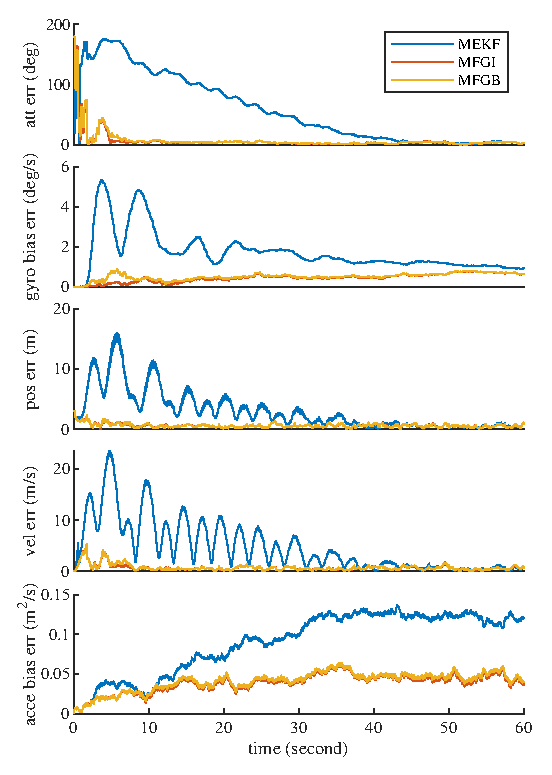
\includegraphics[scale=1.2]{figures/posEst-error}
	\caption{Estimation errors with large initial attitude error.}
	\label{fig:posEst-error}
\end{figure}

\begin{figure}
	\centering
	\begin{subfigure}{\textwidth}
		\centering
		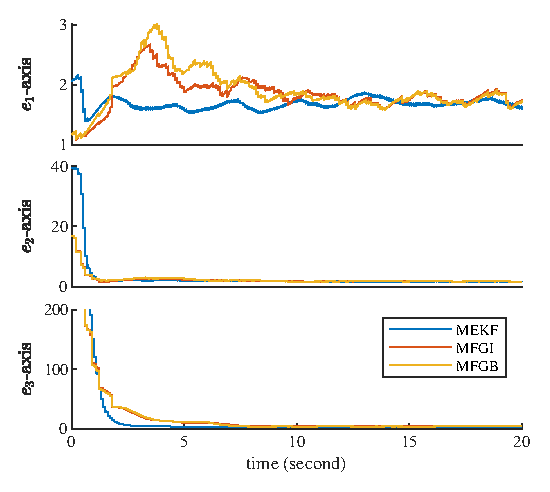
\includegraphics[scale=1.15]{figures/posEst-std-att}
		\caption{Attitude Uncertainty}
		\label{fig:posEst-std-att}
	\end{subfigure}
	\begin{subfigure}{\textwidth}
		\centering
		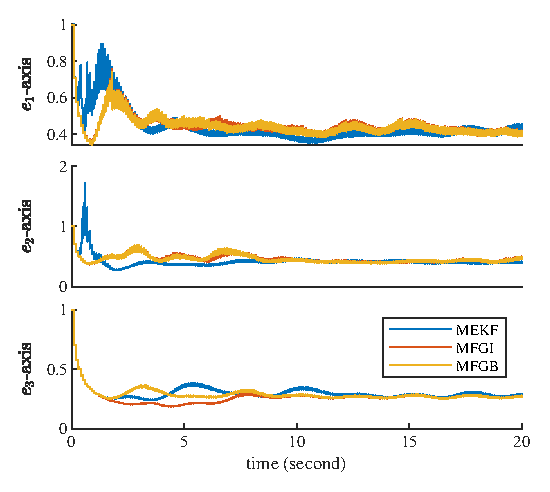
\includegraphics[scale=1.15]{figures/posEst-std-pos}
		\caption{Position Uncertainty}
		\label{fig:posEst-std-pos}
	\end{subfigure}
	\caption[Estimation standard deviations with large initial error.]{Estimation standard deviations with large initial error.
		The attitude standard deviation for MFG is the square root of the diagonals of $U(\tr{S}I_{3\times 3}-S)^{-1}U^T$, and for MEKF is the square root of the diagonals of the covariance matrix transformed into the inertial frame using the estimated attitude.
		And the position standard deviation is the square root of the corresponding entry in the covariance matrix.}
	\label{fig:posEst-std}
\end{figure}

This is more clearly seen in Figure \ref{fig:posEst-std}, where the estimated standard deviations of the attitude and position are shown.
It is seen that although the MEKF has very large attitude error, its uncertainty is on the same level of MFG filters.
Looking at the attitude standard deviation around the gravity direction (the third row in Figure \ref{fig:posEst-std-att}), it converges exponentially for MEKF, which is typical for an EKF.
On the other hand, it converges slower for the MFG filters, possibly indicating that MFG has better accuracy in modeling large attitude uncertainty, as the attitude dose not converge very fast as indicated in Figure \ref{fig:posEst-error}.
Note that in this IMU-GNSS navigation simulation, the attitude is not directly observed, and it is corrected by its correlation with the position.
This suggests that the MFG not only has better accuracy in attitude uncertainty, but also in the correlation between attitude and position, when the attitude uncertainty is large.

\section{Visual-Inertial Odometry} \label{section:VIO}

In this section, the same inertial navigation setting as in the previous section is studied.
But instead of using direct position measurements from GNSS receivers, it is assumed that the 3D coordinates of some unknown features or known landmarks in the inertial frame are measured by cameras.
This is usually referred to as a visual-inertial system.
In this section, two cases are distinguished: (i) if the features captured by the camera are landmarks whose 3D coordinates are known in advance (possibly with noises), it is referred to as visual-inertial \textit{navigation};
(ii) if instead there is no prior information of the features, it is referred to as visual-inertial \textit{odometry}.
To simplify analysis, instead of studying projection measurements on the image plane, it is assumed that the camera is in RGB-D or stereo configuration, so that the 3D coordinates of the feature or landmark in the body-fixed frame are directly measured.
And the measured location is directly used to correct any integration errors from the inertial system.

As reviewed in Chapter \ref{section:intro-review-VIO}, the VIO algorithms can be roughly classified into two categories: filtering and optimization.
The optimization based VIO algorithms have achieved better accuracy, but it is usually more computationally demanding.
This section will primarily focus on the filtering approach.
The reason is that in the optimization method, the uncertainty of pose is not modeled, and the uncertainty for pre-integrated IMU pose is only for a short period of time which is very accurate, so the MFG which is designed to model large uncertainty is not very useful.
On the other hand, the filtering method has to model the uncertainty of pose directly, where large uncertainty is frequently encountered.

More specifically, this section will first study a general problem of estimating a pose and its uncertainty that aligns two 3D point sets with known correspondences.
This is usually one of the steps in point cloud registration \cite{huang2021comprehensive}.
It is first assumed that the 3D coordinates of one point set are perfectly known (map), and the other point set has noises (measurement).
Then based on the proposed algorithm, noises for the map point set are also considered.
The uncertainty of the estimated pose is modeled by MFG to deal with possibly large attitude uncertainties.
Together with the uncertainty propagation method proposed in Chapter \ref{section:posEst-propagation}, these constitute a visual-inertial navigation algorithm when known landmarks in the inertial frame are measured.
Finally, this algorithm is extended to a visual-inertial odometry algorithm where unknown features are measured without any prior information.

\subsection{Pose Estimation Without Map Uncertainty} \label{section:VIO-pose}

First, this subsection studies the problem of finding the pose that aligns two point sets using MFG.
Suppose the coordinates of landmarks in the inertial frame are given as $\{p_i\}_{i=1}^N$.
These are measured by a camera in the body-fixed frame as $\{p'_i\}_{i=1}^N$.
It is assumed that the correspondences are known, i.e., $p'_i$ is the measurement of $p_i$, for $i = 1,\ldots,N$.
The pose of the rigid body is denoted by $(R,t)\in\SE{3}$, where $\SE{3}$ is the three dimensional Euclidean group.
The measurements are affected by noises which are assumed to be zero mean Gaussian, with covariance matrices $A_i$, i.e.,
\begin{align}
	p'_i = R^T(p_i-t) + \mathcal{N}(0,A_i).
\end{align}
To make the calculation easier, the noise $A_i$ is assumed to be isotropic, i.e., $A_i = \sigma_i^2I_{3\times 3}$.
The objective is to find an MFG that describes the uncertainty of the pose $(R,t)$.

The negative log-likelihood function of $(R,t)$ given the point measurements can be written as
\begin{align} \label{eqn:VIO-likelihood}
	f(p'_1,\ldots,p'_N | R,t) = \sum_{i=1}^N \big(R^T(p_i-t)-p'_i\big)^T A_i^{-1} \big(R^T(p_i-t)-p'_i\big).
\end{align}
The conventional method to find $(R,t)$ is to solve the maximum likelihood estimation by posting the above equation into a least square problem, and finding the maximum using Gauss-Newton or Levenberg–Marquardt algorithm.
Denote the Jacobian matrix of the residual error with respect to $(R,t)$ as $J_r\in\mathbb{R}^{3N\times 6}$ in the last step of the optimization, then the covariance of the estimated pose is approximated by $(J_r^TJ_r)^{-1}$.
However, this method is expected to only deal with small uncertainty, and in this subsection \eqref{eqn:VIO-likelihood} is approximated by the exponent of an MFG as in \eqref{eqn:MFG-density}.

As in chapter \ref{section:posEst-update}, the idea is to decompose \eqref{eqn:VIO-likelihood} into two parts: the marginal likelihood of $R$, and the conditional likelihood of $x|R$.
And then the MLE for MFG can be used to recover the parameters from these two likelihood functions.
The approach is motivated by the conventional SVD method \cite{arun1987least,besl1992method}, where the rotation $R$ is first found by centering the two point sets.
This decomposition is formulated in the following theorem.

\begin{theorem} \label{thm:VIO-factor}
	Define $T\in\mathbb{R}^{(N-1)\times N}$ as
	\begin{align}
		T = \begin{bmatrix} 
			\frac{N-1}{N} I_{3\times 3} & \cdots & -\frac{1}{N} I_{3\times 3} & -\frac{1}{N} I_{3\times 3}
			\\ \vdots & \ddots & \vdots & \vdots
			\\ -\frac{1}{N} I_{3\times 3} & \cdots & \frac{N-1}{N} I_{3\times 3} & -\frac{1}{N} I_{3\times 3} 
		\end{bmatrix},
	\end{align}
	and $\mathbf{T} = T\otimes I_{3\times 3} \in \mathbb{R}^{3(N-1)\times 3N}$.
	Denote $\bm{p}'\in\mathbb{R}^{3N\times 1}$ and $\bm{p}_m\in\mathbb{R}^{3N\times 1}$ as the column concatenation of $\{p'_i\}_{i=1}^3$ and $\{R^T(p_i-t)\}_{i=1}^3$, respectively.
	Let $\mathbf{A} = \diag(A_1,\ldots,A_N) \in \mathbb{R}^{3N\times 3N}$ be a block diagonal matrix.
	Also, let $\mathbf{Y} = \Big[ \tfrac{1}{N}I_{3\times 3}, \cdots, \tfrac{1}{N}I_{3\times 3} \Big] \in \mathbb{R}^{3N\times 3}$ be $N$ copies of identity matrices divided by $N$ in a row.
	Define $C\in\mathbb{R}^{3\times 3}$, and $\mathbf{D}\in\mathbb{R}^{3\times 3N}$ as
	\begin{align}
		C &= \mathbf{Y}\mathbf{A}\mathbf{Y}^T - \mathbf{Y}\mathbf{A}\mathbf{T}^T (\mathbf{T}\mathbf{A}\mathbf{T}^T)^{-1} \mathbf{T}\mathbf{A}\mathbf{Y}^T, \label{eqn:VIO-likelihood-C} \\
		\mathbf{D} &= \mathbf{Y}\mathbf{A}\mathbf{T}^T (\mathbf{T}\mathbf{A}\mathbf{T}^T)^{-1} \mathbf{T} - \mathbf{Y}. \label{eqn:VIO-likelihood-D}
	\end{align}
	Let $\mathbf{D}$ be written in block as $\mathbf{D} = \big[D_1, \cdots, D_N\big]$, where $D_i\in\mathbb{R}^{3\times 3}$ for $i=1,\ldots,N$.
	Then, the likelihood \eqref{eqn:VIO-likelihood} can be decomposed as
	\begin{align}
		f(p'_1,\ldots,p'_N | R,t) = f_R(R) + f_{t|R}(t|R),
	\end{align}
	where the marginal likelihood $f_R(R)$ is
	\begin{align} \label{eqn:VIO-likelihood-marginal}
		f_R(R) = (\mathbf{T}\bm{p}'-\mathbf{T}\bm{p}_m)^T \big(\mathbf{T}\mathbf{A}\mathbf{T}^T\big)^{-1} (\mathbf{T}\bm{p}'-\mathbf{T}\bm{p}_m).
	\end{align}
	And the conditional likelihood $f_{t|R}(t|R)$ is
	\begin{align} \label{eqn:VIO-likelihood-conditional}
		f_{t|R}(t|R) = (t - \mu_{t|R})^T (RCR^T)^{-1} (t - \mu_{t|R}),
	\end{align}
	where
	\begin{align} \label{eqn:VIO-likelihood-mu_{t|R}}
		\mu_{t|R} = R \sum_{i=1}^N D_i(p'_i-R^Tp_i).
	\end{align}
\end{theorem}
\begin{proof}
	By definition, \eqref{eqn:VIO-likelihood} can be written as
	\begin{align*}
		f(p'_1,\ldots,p'_N | R,t) = (\bm{p}'-\bm{p}_m)^T \mathbf{A}^{-1} (\bm{p}'-\bm{p}_m).
	\end{align*}
	So it remains to check that
	\begin{align} \label{eqn:VIO-likelihood-conditional-proof}
		f(p'_1,\ldots,p'_N | R,t) - f_R(R) = (\bm{p}'-\bm{p}_m)^T \left( \mathbf{A}^{-1} - \mathbf{T}^T \big(\mathbf{T}\mathbf{A}\mathbf{T}^T\big)^{-1} \mathbf{T} \right) (\bm{p}'-\bm{p}_m)
	\end{align}
	equates $f_{x|R}(x|R)$.
	Let $\mathbf{T}_f = \begin{bmatrix} \mathbf{T} \\ \mathbf{Y} \end{bmatrix}\in\mathbb{R}^{3N\times 3N}$.
	It is straightforward to check that $\mathbf{T}_f$ is full rank and hence invertible.
	So $\mathbf{A}^{-1} = \mathbf{T}_f^T (\mathbf{T}_f\mathbf{A}\mathbf{T}_f^T)^{-1} \mathbf{T}_f$, and
	\begin{align*}
		\mathbf{A}^{-1} - \mathbf{T}^T \big(\mathbf{T}\mathbf{A}\mathbf{T}^T\big)^{-1} \mathbf{T} &= \mathbf{T}_f^T (\mathbf{T}_f\mathbf{A}\mathbf{T}_f^T)^{-1} \mathbf{T}_f - \mathbf{T}^T \big(\mathbf{T}\mathbf{A}\mathbf{T}^T\big)^{-1} \mathbf{T} \\
		&= \begin{bmatrix} \mathbf{T}^T & \mathbf{Y}^T \end{bmatrix} \begin{bmatrix} \mathbf{T}\mathbf{A}\mathbf{T}^T & \mathbf{T}\mathbf{A}\mathbf{Y}^T \\ \mathbf{Y}\mathbf{A}\mathbf{T}^T & \mathbf{Y}\mathbf{A}\mathbf{Y}^T\end{bmatrix}^{-1} \begin{bmatrix} \mathbf{T} \\ \mathbf{Y} \end{bmatrix} - \mathbf{T}^T \big(\mathbf{T}\mathbf{A}\mathbf{T}^T\big)^{-1} \mathbf{T} \\
		&= \mathbf{D}^T C^{-1} \mathbf{D},
	\end{align*}
	where the last equality uses the block inversion formula \cite{petersen2008matrix}.
	Note that $\mathbf{TY}^T = 0$, so
	\begin{align*}
		\sum_{i=1}^N D_i = N\mathbf{DY}^T = N\mathbf{YAT}^T (\mathbf{TAT}^T)^{-1} \mathbf{TY}^T - N\mathbf{YY}^T = -N\mathbf{YY}^T = -I_{3\times 3}.
	\end{align*}
	Next, it can be shown that
	\begin{align*}
		\mathbf{D}(\bm{p}' - \bm{p}_m) &= \sum_{i=1}^N D_i(p'_i - R^Tp_i + R^Tt) \\
		&= -R^Tt - \sum_{i=1}^N D_iR^Tp_i + \sum_{i=1}^N D_ip'_i \\
		&= -R^T\left( t - R\sum_{i=1}^N D_i(p'_i-R^Tp_i) \right).
	\end{align*}
	Substitute these into \eqref{eqn:VIO-likelihood-conditional-proof} yields $f(p'_1,\ldots,p'_N | R,t) - f_R(R) = f_{x|R}(x|R)$.
\end{proof}

With this decomposition of the likelihood \eqref{eqn:VIO-likelihood}, the marginal part $f_R(R)$ can be first approximated by a matrix Fisher density, then the conditional part $f_{x|R}(x|R)$ can be use in Theorem \ref{thm:MFG-MLE-conditional} to recover the parameters $\mu$, $\Sigma$, and $P$ of the MFG.

\paragraph{Marginal Likelihood}

First, an algorithm to approximate the marginal likelihood \eqref{eqn:VIO-likelihood-marginal} is developed.
Define $q_i$, $q'_i\in\mathbb{R}^3$ for $i = 1,\ldots,N-1$ as
\begin{align} \label{eqn:VIO-centering}
	q_i = p_i-\frac{1}{N} \sum_{i=1}^N p_i, \qquad\qquad q'_i = p'_i - \frac{1}{N} \sum_{i=1}^N p'_i,
\end{align}
i.e., they are $\{p_i\}$ and $\{p'_i\}$ centered by their geometric centers.
Define $\bm{q'}\in\mathbb{R}^{3(N-1)\times 1}$ and $\bm{q}_m\in\mathbb{R}^{3(N-1)\times 1}$ as the concatenation of $\{q'_i\}_{i=1}^{N-1}$ and $\{R^Tq_i\}_{i=1}^{N-1}$ respectively.
It is straightforward to verify that $\bm{q}' = \mathbf{T}\bm{p}'$, and $\bm{q}_m = T\bm{p}_m$.
Note that the translation $t$ in $\bm{p}_m$ does not appear in the centered $\bm{q}_m$ anymore, which is the key point that $f_R(R)$ does not depend on $t$.
With these notations, the marginal likelihood \eqref{eqn:VIO-likelihood-marginal} can be written as
\begin{align} \label{eqn:VIO-likelihood-marginal-q}
	f_R(R) = (\bm{q}'-\bm{q}_m)^T \big(\mathbf{T}\mathbf{A}\mathbf{T}^T\big)^{-1} (\bm{q}'-\bm{q}_m).
\end{align}

Now finding the $R\in\SO{3}$ that maximizes $f_R(R)$ becomes very similar to the classic Wahba's problem \cite{markley1988attitude,shuster1981three}.
In other words, $q'_i$ can be regarded as direction measurements of $q_i$, for $i=1,\ldots,N-1$, and $R$ can be found by aligning these two sets of directions.
However, the difficulty is that $q'_i$ are correlated, since $\mathbf{T}\mathbf{A}\mathbf{T}^T$ in general has nonzero diagonal terms.
Two cases are considered here: (i) all measurements have equal covariance matrices, i.e. $A_1 = \cdots = A_N$, and (ii) the covariance matrices are different.
It is firstly shown that for equal covariance matrices, a linear transform can be applied to $\{q_i\}_{i=1}^{N-1}$ again to make them uncorrelated, so $R$ can be found using an algorithm similar to Theorem III.2 in \cite{lee2018bayesian}.

\begin{theorem}
	The matrix $TT^T \in \mathbb{R}^{(N-1)\times (N-1)}$ is invertible.
	Let $TT^T = U^TDU$ be the eigen-decomposition of $TT^T$.
	For $i = 1,\ldots,N-1$, let
	\begin{align} \label{eqn:VIO-uncorrelate}
		r_i = \sum_{j=1}^{N-1} U_{ij} q_i \qquad\qquad r'_i = \sum_{j=1}^{N-1} U_{ij} q'_i,
	\end{align}
	where $U_{ij}$ is the $(i,j)$-th entry of $U$.
	If $A_1 = \cdots = A_N \triangleq A = \sigma^2I_{3\times 3}$, then
	\begin{align} \label{eqn:VIO-likelihood-marginal-r}
		f_R(R) = (\bm{r}'-\bm{r}_m)^T (D\otimes A)^{-1} (\bm{r}'-\bm{r}_m),
	\end{align}
	where $\bm{r}'$ and $\bm{r}_m$ are the concatenation of $\{r'_i\}_{i=1}^{N-1}$ and $\{R^T r_i\}_{i=1}^{N-1}$ respectively.
\end{theorem}
\begin{proof}
	The invertibility of $TT^T \in \mathbb{R}$ can be verified by direction calculation.
	Also, it can be easily shown that $\bm{r}' = (U\otimes I_{3\times 3}) \bm{q}'$, and $\bm{r}_m = (U\otimes I_{3\times 3})\bm{q}_m$.
	Note that $(U\otimes I_{3\times 3})^{-1} = U^T\otimes I_{3\times 3} = (U\otimes I_{3\times 3})^T$, so $\bm{q}' = (U\otimes I_{3\times 3})^T \bm{r}'$, and $\bm{q}_m = (U\otimes I_{3\times 3})^T \bm{r}_m$.
	Then by \eqref{eqn:VIO-likelihood-marginal-q}, $f_R(R)$ can be written as
	\begin{align*}
		f_R(R) = (\bm{r}'-\bm{r}_m)^T (U\otimes I_{3\times 3}) \big(\mathbf{T}\mathbf{A}\mathbf{T}^T\big)^{-1} (U\otimes I_{3\times 3})^T (\bm{r}'-\bm{r}_m).
	\end{align*}
	Because $\mathbf{T}\mathbf{A}\mathbf{T}^T = (T\otimes I_{3\times 3})(I_{N\times N}\otimes A)(T\otimes I_{3\times 3})^T$, the covariance matrix for $\bm{r}'$ becomes
	\begin{align*}
		&(U\otimes I_{3\times 3}) \big(\mathbf{T}\mathbf{A}\mathbf{T}^T\big)^{-1} (U\otimes I_{3\times 3})^T \\
		= &\left( (U\otimes I_{3\times 3}) (T\otimes I_{3\times 3}) (I_{N\times N}\otimes A) (T\otimes I_{3\times 3})^T (U\otimes I_{3\times 3})^T \right)^{-1} \\
		= &\left( (UT\otimes I_{3\times 3}) (I_{N\times N}\otimes A) (UT\otimes I_{3\times 3})^T \right)^{-1} \\
		= &(UTT^TU^T \otimes A)^{-1} \\
		= &(D\otimes A)^{-1}.
	\end{align*}
	And \eqref{eqn:VIO-likelihood-marginal-r} is obtained.
\end{proof}

Since $D = \diag(d_1,\ldots d_{N-1})$ is a diagonal matrix, only the diagonal blocks of $D\otimes A$ is nonzero.
Therefor, the marginal likelihood \eqref{eqn:VIO-likelihood-marginal-r} can be treated as measuring $N-1$ directions $r_i$ in the inertial frame with noises.
More specifically, the measurements $r'_i$ can be written as
\begin{align} \label{eqn:VIO-direction-measurement}
	r'_i = R^Tr_i + \mathcal{N}(0, d_i\sigma^2 I_{3\times 3}),
\end{align}
for $i = 1,\ldots,N-1$.
To approximate \eqref{eqn:VIO-likelihood-marginal-r} into a matrix Fisher density, the Gaussian distribution of $r'_i$ is first approximated by a von Mises--Fisher distribution on $\Sph^2$ according to the following lemma.

\begin{lemma} \label{thm:VIO-GaussToVM}
	The density function of $\tfrac{r'_i}{\norm{r'_i}}$ in \eqref{eqn:VIO-direction-measurement} can be approximated by
	\begin{align} \label{eqn:VIO-direction-vonMises}
		p\left( \tfrac{r'_i}{\norm{r'_i}} \right) \approx c \expb{\kappa_i \tfrac{(r')_i^TR^Tr_i}{\norm{r'_i}\norm{r_i}}}
	\end{align}
	where $c$ is a normalizing constant. The concentration parameter $\kappa_i$ is solved from
	\begin{align} \label{eqn:VIO-resultantLenth}
		\coth\kappa_i - \frac{1}{\kappa_i} = \frac{2}{\gamma} \phi(\gamma) + \left( 1-\frac{1}{\gamma^2} \right) (2\Phi(\gamma)-1),
	\end{align}
	where $\gamma = \norm{r_i}/(\sqrt{d_i}\sigma)$, $\phi(\cdot)$ and $\Phi(\cdot)$ are the probability density and cumulative density functions of the one dimensional normal distribution.
\end{lemma}
\begin{proof}
	Because $r'_i$ follows a Gaussian distribution, its direction $r'_i/\norm{r'_i}$ follows a projected normal distribution \cite{mardia2009directional}.
	And its mean resultant length \cite{presnell2008mean} can be calculated as on the right hand side of \eqref{eqn:VIO-resultantLenth}.
	Based on the maximum likelihood estimation \cite{mardia2009directional} for a von Mises--Fisher distribution, $r'_i/\norm{r'_i}$ can be matched to a von Mises--Fisher distribution with mean direction $R^Tr_i/\norm{r_i}$, and the concentration parameter solved from \eqref{eqn:VIO-resultantLenth}.
	The density function is given in \eqref{eqn:VIO-direction-vonMises}.
\end{proof}

Based on the above lemma, the marginal likelihood $f_R(R)$ in \eqref{eqn:VIO-likelihood-marginal-r} can be further approximated by
\begin{align} \label{eqn:VIO-likelihood-marginal-F}
	\expb{-\tfrac{1}{2}f_R(R)} &\approx c \sum_{i=1}^{N-1} \expb{\kappa_i \tfrac{(r')_i^TR^Tr_i}{\norm{r'_i}\norm{r_i}}} \nonumber \\ 
	&= c \cdot \etr{\left(\sum_{i=1}^{N-1} \kappa_i \tfrac{r_i(r'_i)^T}{\norm{r_i}\norm{r'_i}}\right) R^T} \triangleq c \cdot \etr{FR^T},
\end{align}
for some constant $c$.
In other words, the marginal likelihood $f_R(R)$ is matched to a matrix Fisher density with the parameter $F = \sum_{i=1}^{N-1} \kappa_i \tfrac{r_i(r'_i)^T}{\norm{r_i}\norm{r'_i}}$.

Nevertheless, the approximation in \eqref{eqn:VIO-likelihood-marginal-F} requires that all measurements have the same isotropic noise $A = \sigma^2I_{3\times 3}$, which seems too stringent.
To relax this requirement such that the measurements can have different levels of noises $A_i = \sigma_i^2 I_{3\times 3}$, the technique of \textit{importance sampling} is used.
Similar to Chapter \ref{section:posEst-update}, the idea is to use unscented transform to select sigma points from a matrix Fisher distribution, and reweigh these sigma points to calculated the expectation $\expect{R}$ according to the density function \eqref{eqn:VIO-likelihood-marginal-q}.
To use importance sampling, a \textit{proposal} matrix Fisher distribution is needed that is close to the density function \eqref{eqn:VIO-likelihood-marginal-q}.
A good choice is simply treating $\{q'_i\}_{i=1}^{N-1}$ as uncorrelated direction measurements, and using Theorem \ref{thm:VIO-GaussToVM} and \eqref{eqn:VIO-likelihood-marginal-F} to find a matrix Fisher distribution.

Let this matrix Fisher distribution be denoted by $\mathcal{M}(F_\text{prop})$, and its density function be denoted by $f_\text{prop}(R)$.
Select sigma points \cite{gilitschenski2015unscented,lee2018bayesian} $\{(R_j,w_j)\}_{j=1}^7$ from the proposal distribution $\mathcal{M}(F_\text{prop})$, and reweigh these sigma points as
\begin{align} \label{eqn:VIO-update-sigmapoints}
	w_j^+ = w_j \cdot \frac{\expb{-\tfrac{1}{2}f_R(R_j)}}{f_\text{prop}(R_j)}.
\end{align}
Then the reweighed sigma points $\{(R_j,w_j^+)\}_{j=1}^7$ can be regarded as weighted samples from the density \eqref{eqn:VIO-likelihood-marginal-q}.
And the expectation $\expect{R}$ can be calculated as $\expect{R} = \sum_{j=1} w_j^+R_j$ after normalization, which can be matched to a matrix Fisher distribution using the MLE as introduced in Chapter \ref{section:MF-MF}.

Note that the update of weights in \eqref{eqn:VIO-update-sigmapoints} is similar to that in \eqref{eqn:posEst-update-sigmapoints}, so the progressive update procedure in Chapter \ref{section:posEst-update} can also be used here to improve accuracy.
In addition, even if all measurements have the same covariance matrix, \eqref{eqn:VIO-likelihood-marginal-F} is still not perfect due to the approximation of projected normal distribution as von Mises--Fisher distribution in Theorem \ref{thm:VIO-GaussToVM}.
So using this importance sampling approach with \eqref{eqn:VIO-likelihood-marginal-F} as the proposal distribution is also expected to improve accuracy even for the case of same covariance matrix.
The pseudocode to match \eqref{eqn:VIO-likelihood-marginal} to a matrix Fisher density is given in Table \ref{tab:VIO-marginal}.

\begin{table}
	\caption{Attitude Estimation From Marginal Likelihood}
	\label{tab:VIO-marginal}
	\begin{algorithmic}[1]
		\algrule[0.8pt]
		\Procedure{$F = $ Attitude Estimation}{$\{p_i\}$, $\{p'_i\}$}
		\algrule
		\State Calculate $\{q_i\}$ and $\{q'_i\}$ using \eqref{eqn:VIO-centering}.
		\If{$A_1 = \cdots = A_N$}
		\State Calculate $\{r_i\}$ and $\{r'_i\}$ using \eqref{eqn:VIO-uncorrelate}.
		\State Calculate $F_\text{prop}$ as in \eqref{eqn:VIO-likelihood-marginal-F} using Theorem \ref{thm:VIO-GaussToVM}.
		\Else
		\State Calculate $F_\text{prop}$ as in \eqref{eqn:VIO-likelihood-marginal-F} using Theorem \ref{thm:VIO-GaussToVM}, with $\{r_i\}$ and $\{r'_i\}$ replaced by $\{q_i\}$ and $\{q'_i\}$, and $d_i\sigma^2I_{3\times 3}$ in \eqref{eqn:VIO-direction-measurement} replaced by the $i$-th diagonal block of $\mathbf{TAT}^T$.
		\EndIf
		\State Select sigma points \cite{gilitschenski2015unscented,lee2018bayesian} from $\mathcal{M}(F_\text{prop})$ as $\{R_j,w_j\}_{j=1}^7$.
		\State Let $\lambda = 1$.
		\While{$\lambda > 0$}
		\State For $j=1,\ldots,7$, calculate $f_m(R_j)^\lambda$, with $f_m(R) = \expb{-\tfrac{1}{2}f_R(R)} / f_\text{prop}(R)$, where $f_R(R)$ is in \eqref{eqn:VIO-likelihood-marginal-q}, and $f_\text{prop}$ is the density function of $\mathcal{M}(F_\text{prop})$.
		\If{$\min\{f_m(R_j)^{\lambda}\} / \max\{f_m(R_j)^{\lambda}\} < \tau$}
		\State Let $\alpha = \log\tau / \log\left( \tfrac{\min\{f_m(R_j)\}}{\max\{f_m(R_j)\}} \right)$.
		\State For $j=1,\ldots,7$, calculate $f_m(R_j)^\alpha$.
		\State For $j=1,\ldots,7$, update the weights as $w_j^+ = w_j f_m(R_j)^\alpha$.
		\State Normalize the weights as $w_j^+ = w_j^+/\sum_{j=1}^7 w_j^+$.
		\State Calculate $\expect{R} = \sum_{i=j}^7 w_i^+ R_j$.
		\State Select sigma points $\{R_j,w_j\}_{j=1}^7$ from the matrix Fisher distribution that has the moment $\expect{R}$.
		\State Set $\lambda = \lambda-\alpha$.
		\Else
		\State Set $\lambda = 0$.
		\EndIf
		\EndWhile
		\State For $j=1,\ldots,7$, update the weights as $w_j^+ = w_j f_m(R_j)^\lambda$.
		\State Normalize the weights as $w_j^+ = w_j^+/\sum_{j=1}^7 w_j^+$.
		\State Calculate $\expect{R} = \sum_{j=1}^7 w_j^+ R_j$.
		\State Obtain $F$ using the MLE of matrix Fisher distribution in Chapter \ref{section:MF-MF} from $\expect{R}$.
		\EndProcedure
		\algrule[0.8pt]
	\end{algorithmic}
\end{table}

In summary, after matching the marginal likelihood \eqref{eqn:VIO-likelihood-marginal} to a matrix Fisher distribution with parameter $F$, the full likelihood \eqref{eqn:VIO-likelihood} has been approximated by
\begin{align} \label{eqn:VIO-likelihood-approx}
	\expb{-\tfrac{1}{2}f(p'_1,\ldots,p'_N|R,t)} \approx c\cdot \etr{FR^T} \expb{-\tfrac{1}{2}f_{x|R}(x|R)},
\end{align}
where $c$ is a normalizing constant, and $f_{x|R}(x|R)$ is the conditional likelihood \eqref{eqn:VIO-likelihood-conditional}.
In the next subsection, the conditional likelihood \eqref{eqn:VIO-likelihood-conditional} is further used to match \eqref{eqn:VIO-likelihood-approx} to an MFG density.

\paragraph{Conditional Likelihood}

As before, the conditional likelihood is handled by the conditional MLE of MFG in Theorem \ref{thm:MFG-MLE-conditional}.
After obtaining $F$ from the marginal likelihood, let $F = USV^T$ be its pSVD, and define $\nu_R = (QS-SQ^T)^\vee$ for MFGI, or $\nu_R = (SQ-Q^TS)^\vee$ for MFGB, with $Q = U^TRV$.
To use the theorem, the following moments needs to be calculated: $\expect{t}$, $\expect{t\nu_R^T}$, and $\expect{tt^T}$.
These moments are according to the density function \eqref{eqn:VIO-likelihood-approx}.
As shown in \eqref{eqn:VIO-likelihood-mu_{t|R}}, clearly $\expect{tt^T}$ involves the fourth order of $R$, which currently do not have closed form formulae.
To simplify these moments, the follow lemma is very useful.

\begin{lemma} \label{lemma:VIO-likelihood-CD}
	Given $A_i = \sigma_i^2I_{3\times 3}$ for $i=1,\ldots,N$, $C$ in \eqref{eqn:VIO-likelihood-C} and $\mathbf{D}$ in \eqref{eqn:VIO-likelihood-D} satisfy the following equations:
	\begin{align}
		RCR^T &= C, \label{eqn:VIO-likelihood-C-sim} \\
		RD_iR^T &= D_i. \label{eqn:VIO-likelihood-D-sim}
	\end{align}
\end{lemma}
\begin{proof}
	Note that $R\mathbf{Y} = \mathbf{Y}(I_{N\times N}\otimes R)$, and $(I_{N\times N}\otimes R) \mathbf{A} (I_{N\times N}\otimes R)^T = \diag(RA_1R^T,\allowbreak \ldots,\allowbreak RA_NR^T) = \mathbf{A}$.
	For $C$, it can be shown that
	\begin{align*}
		R\mathbf{YAY}^TR^T &= \mathbf{Y} (I_{N\times N}\otimes R) \mathbf{A} (I_{N\times N}\otimes R)^T \mathbf{Y}^T = \mathbf{YAY}^T.
	\end{align*}
	Also, note that $\left(I_{(N-1)\times (N-1)}\otimes R\right) \mathbf{T} = \mathbf{T} (I_{N\times N}\otimes R)$, and $(I_{N\times N}\otimes R)^T \mathbf{A} (I_{N\times N}\otimes R) = \mathbf{A}$, so the following equality holds:
	\begin{align*}
		\mathbf{TAT}^T = \left(I_{(N-1)\times (N-1)}\otimes R\right)^T \mathbf{TAT}^T \left(I_{(N-1)\times (N-1)}\otimes R\right).
	\end{align*}
	Therefore, it can be shown that
	\begin{align*}
		&R\mathbf{Y}\mathbf{A}\mathbf{T}^T (\mathbf{T}\mathbf{A}\mathbf{T}^T)^{-1} \mathbf{T}\mathbf{A}\mathbf{Y}^TR^T \\
		= &R\mathbf{Y} \mathbf{AT}^T \left(I_{(N-1)\times (N-1)}\otimes R\right)^T (\mathbf{TAT}^T)^{-1} \left(I_{(N-1)\times (N-1)}\otimes R\right) \mathbf{TA} \mathbf{Y}^T R^T \\
		= &R\mathbf{YA} (I_{N\times N}\otimes R)^T \mathbf{T}^T (\mathbf{TAT}^T)^{-1} \mathbf{T} (I_{N\times N}\otimes R) \mathbf{AY}^T R \\
		= &R\mathbf{Y} (I_{N\times N}\otimes R)^T \mathbf{AT}^T (\mathbf{TAT}^T)^{-1} \mathbf{TA} (I_{N\times N}\otimes R) \mathbf{Y}^T R \\
		= &\mathbf{Y}\mathbf{A}\mathbf{T}^T (\mathbf{T}\mathbf{A}\mathbf{T}^T)^{-1} \mathbf{T}\mathbf{A}\mathbf{Y}^T,
	\end{align*}
	which proves \eqref{eqn:VIO-likelihood-C-sim}.
	Equation \eqref{eqn:VIO-likelihood-D-sim} can be proved using similar calculations.
\end{proof}

With the above lemma, the conditional likelihood \eqref{eqn:VIO-likelihood-conditional} with its conditional mean \eqref{eqn:VIO-likelihood-mu_{t|R}} is now simplified as
\begin{align} \label{eqn:VIO-likelihood-conditional-sim}
	f_{t|R}(t|R) = \left( t - \sum_{i=1}^N D_i(Rp'_i - p_i) \right)^T C^{-1} \left( t - \sum_{i=1}^N D_i(Rp'_i - p_i) \right).
\end{align}
Then the moments required for the conditional MLE of MFG are evaluated as follows:

\begin{theorem} \label{thm:VIO-conditional}
	The moments $\expect{t}$, $\expect{t\nu_R^T}$, and $\expect{tt^T}$ according to the density \eqref{eqn:VIO-likelihood-approx} are
	\begin{align}
		\expect{t} &= \sum_{i=1}^N D_i(\expect{R}p'_i-p_i), \\
		\expect{t\nu_R^T} &= \sum_{i=1}^N D_i \expect{Rp'_i\nu_R^T}, \\
		\expect{tt^T} &= C + \sum_{i=1}^N \sum_{j=1}^N D_i \left( \expect{Rp'_i(p'_j)^TR^T} - \expect{R}p'_ip_j^T - p_i(p'_j)^T\expect{R}^T + p_ip_j^T \right) D_j^T. \label{eqn:VIO-likelihood-Ett}
	\end{align}
\end{theorem}
\begin{proof}
	These equations can be easily derived by integrating the left hand side with respect to the Gaussian density \eqref{eqn:VIO-likelihood-conditional-sim} first, as in \eqref{eqn:MFG-Exx-proof}.
\end{proof}

It is notable that the complexity for $\expect{tt^T}$ in \eqref{eqn:VIO-likelihood-Ett} is $O(N^2)$, which becomes computationally demanding if the number of points is large.
This cannot be avoided for general cases, but in next theorem, it is shown that if all measurements have the same covariance matrices, the expressions for $\expect{t}$, $\expect{t\nu_R^T}$, and $\expect{tt^T}$ can be greatly simplified.

\begin{theorem} \label{thm:VIO-conditional-sim}
	Let $p_c = \tfrac{1}{N}\sum_{i=1}^N p_i$, and $p'_c = \tfrac{1}{N}\sum_{i=1}^N p'_i$.
	If $A_1 = \cdots = A_N \triangleq A = \sigma^2I_{3\times 3}$, then $\expect{t}$, $\expect{t\nu_R^T}$, and $\expect{tt^T}$ according to the density \eqref{eqn:VIO-likelihood-approx} are
	\begin{align}
		\expect{t} &= p_c - \expect{R}p'_c \\
		\expect{t\nu_R^T} &= -\expect{Rp'_c\nu_R^T} \\
		\expect{tt^T} &= \tfrac{\sigma^2}{N}I_{3\times 3} + \expect{Rp'_c(p'_c)^TR^T} - p_c(p'_c)^T\expect{R}^T - \expect{R}p'_cp_c^T + p_cp_c^T.
	\end{align}
\end{theorem}
\begin{proof}
	Let $Y = \tfrac{1}{N}[1,\ldots,1]\in\mathbb{R}^{1,N}$ so that $\mathbf{Y} = Y\otimes I_{3\times 3}$.
	Note that $YT^T = 0$, so it can be shown that
	\begin{align*}
		\mathbf{YAT}^T = (Y\otimes I_{3\times 3})(I_{N\times N}\otimes A) (T^T\otimes I_{3\times 3}) = YT^T\otimes A = 0.
	\end{align*}
	So $C = \mathbf{YAY}^T = \tfrac{1}{N}A = \tfrac{\sigma^2}{N} I_{3\times 3}$, and $\mathbf{D} = -\mathbf{Y}$, i.e., $D_i = -\tfrac{1}{N}I_{3\times 3}$ for $i=1,\ldots,N$.
	Substitute these into \eqref{eqn:VIO-likelihood-conditional-sim}, it is simplified to
	\begin{align}
		f_{t|R}(t|R) = \left( t - (p_c-Rp'_c) \right)^T \left( \tfrac{\sigma^2}{N}I_{3\times 3} \right)^{-1} \left( t - (p_c-Rp'_c) \right),
	\end{align}
	and the desired moments can be easily derived.
\end{proof}

After calculating the moments $\expect{t}$, $\expect{t\nu_R^T}$, and $\expect{tt^T}$, they can be used in the conditional MLE for MFG to obtain the parameters $\mu$, $\Sigma$, and $P$.
So the likelihood function \eqref{eqn:VIO-likelihood} is matched to an MFG.
The pseudocode is summarized in Table \ref{tab:VIO-pose}.

\begin{table}
	\caption{Pose estimation without map noises}
	\label{tab:VIO-pose}
	\begin{algorithmic}[1]
		\algrule[0.8pt]
		\Procedure{$\mathcal{MG} = $ Pose Estimation}{$\{p_i\}$, $\{p'_i\}$}
		\algrule
		\State Obtain $F=$ Attitude Estimation($\{p_i\}$, $\{p'_i\}$) in Table \ref{tab:VIO-marginal}.
		\State Let $F = USV^T$ be its pSVD.
		\State Calculate $\expect{\nu_R\nu_R^T}$ as in \eqref{eqn:MFG-EvRvR} using $S$.
		\If{$A_1 = \cdots = A_N$}
		\State Calculate $\expect{t}$, $\expect{t\nu_R^T}$, and $\expect{tt^T}$ in Theorem \ref{thm:VIO-conditional-sim}.
		\Else
		\State Calculate $\expect{t}$, $\expect{t\nu_R^T}$, and $\expect{tt^T}$ in Theorem \ref{thm:VIO-conditional}.
		\EndIf
		\State Obtain $\mu$, $\Sigma$, $P$ according to Theorem \ref{thm:MFG-MLE-conditional}, with $\expect{t}$, $\expect{t\nu_R^T}$, $\expect{tt^T}$, $\expect{\nu_R\nu_R^T}$, and $\expect{\nu_R} = 0$.
		\State Set $\mathcal{MG} = \mathcal{MG}(\mu,\Sigma,P,U,S,V)$.
		\EndProcedure
		\algrule[0.8pt]
	\end{algorithmic}
\end{table}

\paragraph{Posterior Density}

Up to Table \eqref{tab:VIO-pose}, an algorithm to find the distribution of the pose $(R,t)$ modeled by MFG is given to align the map point set $\{p_i\}$ and measurement point set $\{p'_i\}$.
If this algorithm is used in a filtering algorithm, the pose also has a prior distribution.
Here a more general problem is considered.
Let $y = [t^T, a^T]^T \in \mathbb{R}^n$, suppose $(R,y)$ follows an MFG with the parameter $(\mu,\Sigma,P,U,S,V)$ before measurements, where $a$ includes other Euclidean quantities, such as linear velocity and sensor biases as in the IMU-GNSS navigation.
According to the Bayes' formula, the posterior density for $(R,y)$ after incorporating the measurements $\{p'_i\}$ is
\begin{align} \label{eqn:VIO-posterior}
	p(R,y|p'_1,\ldots,p'_N) &\propto p(p'_1,\ldots,p'_N|R,t) p(R,y) \nonumber \\
	&= \expb{-\tfrac{1}{2}\sum_{i=1}^N \big(R^T(p_i-Hy)-p'_i\big)^T A_i^{-1} \big(R^T(p_i-Hy)-p'_i\big)} \nonumber \\
	&\qquad \cdot \etr{FR^T} \expb{-\tfrac{1}{2}(y-\mu_c)^T \Sigma_c^{-1} (y-\mu_c)},
\end{align}
where the first exponential term on the right hand side is the likelihood \eqref{eqn:VIO-likelihood}, with $H = [I_{3\times 3}, 0_{3\times (n-3)}]$ selects $t$ from $y$.
The intermediate parameters $F$, $\mu_c$, and $\Sigma_c$ are defined with respect to $\mathcal{MG}(\mu,\Sigma,P,U,S,V)$.
Next, matching the posterior density $p(R,y|p'_1,\ldots,p'_N)$ to an MFG is studied.

In Theorem \ref{thm:VIO-factor}, the likelihood $f(p'_1,\ldots,p'_N|R,t)$ has been factorized into the marginal $f_R(R)$ and the conditional $f_{x|R}(x|R)$, which can be directly applied to the posterior density.
\begin{align} \label{eqn:VIO-posterior-factor1}
	&p(R,y|p'_1,\ldots,p'_N) \propto \expb{FR^T} \expb{-\tfrac{1}{2}(\bm{q}'-\bm{q}_m)^T \big(\mathbf{T}\mathbf{A}\mathbf{T}^T\big)^{-1} (\bm{q}'-\bm{q}_m)} \nonumber \\
	&\qquad \cdot \expb{-\tfrac{1}{2}(y-\mu_c)^T \Sigma_c^{-1} (y-\mu_c)} \expb{-\tfrac{1}{2}(Hy - \mu_{t|R})^T C^{-1} (Hy - \mu_{t|R})}
\end{align}
with $\mu_{t|R}$ given as in \eqref{eqn:VIO-likelihood-conditional-sim}.
The last two terms has the same structure as in \eqref{eqn:posEst-update-density}, so they can be calculated similarly as in Lemma \ref{lemma:posEst-update-factor}.
More specifically, define
\begin{align}
	K = \Sigma_cH^T(H\Sigma_cH^T + C)^{-1}.
\end{align}
Then \eqref{eqn:VIO-posterior-factor1} can be further factorized into
\begin{align} \label{eqn:VIO-posterior-factor2}
	&p(R,y|p'_1,\ldots,p'_N) \propto \expb{FR^T} \expb{-\tfrac{1}{2}(\bm{q}'-\bm{q}_m)^T \big(\mathbf{T}\mathbf{A}\mathbf{T}^T\big)^{-1} (\bm{q}'-\bm{q}_m)} \nonumber \\
	&\qquad \cdot \expb{-\tfrac{1}{2} (H\mu_c-\mu_{t|R})^T (C + H\Sigma_cH^T)^{-1} (H\mu_c-\mu_{t|R})^T} \nonumber \\
	&\qquad \cdot \expb{-\tfrac{1}{2} (y-(I-KH)\mu_c-K\mu_{t|R})^T \big((I-KH)\Sigma_c\big)^{-1} (y-(I-KH)\mu_c-K\mu_{t|R})},
\end{align}
where $I$ is an abbreviation of $I_{n\times n}$.
The first three terms on the right hand side of \eqref{eqn:VIO-posterior-factor2} do not depend on $y$, and they can be regarded as the marginal posterior density for $R$.
The same algorithm as in Table \ref{tab:posEst-update-att} can be used to approximate it to a matrix Fisher distribution.
Let the approximated parameter be denoted by $F^+$, then \eqref{eqn:VIO-posterior-factor2} is approximated by
\begin{align} \label{eqn:VIO-posterior-approx}
	&p(R,y|p'_1,\ldots,p'_N) \propto \expb{F^+R^T} \cdot p_{y|R}(y|R),
\end{align}
where $p_{y|R}(y|R)$ is the last term in \eqref{eqn:VIO-posterior-factor2}.

Let $F^+ = U^+S^+(V^+)^T$ be its pSVD, define $\nu_R^+ = (Q^+S^+ - S^+(Q^+)^T)^\vee$ for MFGI, or $\nu_R^+ = (S^+Q^+ - (Q^+)^TS^+)^\vee$ for MFGB, with $Q^+ = (U^+)^TS^+V^+$.
The function $p_{y|R}(y|R)$ is Gaussian for $y$, and it can be regarded as the conditional posterior density for $y|R$.
To use the conditional MLE of MFG, the moments $\expect{y}$, $\expect{y(\nu_R^+)^T}$, and $\expect{yy^T}$ according to the density \eqref{eqn:VIO-posterior-approx} need to be calculated.
To distinguish these moments with those moments according to the prior $\mathcal{MG}(\mu,\Sigma,P,U,S,V)$, they are denoted by $\expect{y|\mathcal{Z}}$, $\expect{y(\nu_R^+)^T|\mathcal{Z}}$, and $\expect{yy^T|\mathcal{Z}}$, where $\mathcal{Z} = \{p'_i\}_{i=1}^N$ are all measurements.

\begin{table}
	\caption{Measurement update without map noises}
	\label{tab:VIO-update}
	\begin{algorithmic}[1]
		\algrule[0.8pt]
		\Procedure{$\mathcal{MG}^+$ = Measurement Update}{$\mathcal{MG}^-$, $\{p_i\}$, $\{p'_i\}$}
		\algrule
		\State Let $F^- = U^-S^-(V^-)^T$.
		\State Calculate $F^+=$ Attitude Update($F^-$, $\{p_i\}$, $\{p'_i\}$).
		\State Let the pSVD of $F^+$ be $F^+ = U^+S^+(V^+)^T$.
		\State Calculate the moments of the posterior density in Theorem \ref{thm:VIO-posterior-conditional-moments}.
		\State Obtain $\mu^+$, $\Sigma^+$, and $P^+$ using the conditional MLE in Theorem \ref{thm:MFG-MLE-conditional}.
		\State Set $\mathcal{MG}^+ = \mathcal{MG}(\mu^+,\Sigma^+,P^+,U^+,S^+,V^+)$.
		\EndProcedure
		\algrule
		\Procedure{$F^+ = $ Attitude Update}{$F^-$, $\{p_i\}$, $\{p'_i\}$}
		\State Select sigma points \cite{gilitschenski2015unscented,lee2018bayesian} from $\mathcal{M}(F^-)$ as $\{R_j,w_j\}_{j=1}^7$.
		\State Let $\lambda = 1$.
		\While{$\lambda > 0$}
		\State For $j=1,\ldots,7$, calculate $f_m(R_j)^\lambda$, where $f_m(R)$ is the second and third terms on the right hand side of \eqref{eqn:VIO-posterior-factor2}.
		\If{$\min\{f_m(R_j)^{\lambda}\} / \max\{f_m(R_j)^{\lambda}\} < \tau$}
		\State Let $\alpha = \log\tau / \log\left( \tfrac{\min\{f_m(R_j)\}}{\max\{f_m(R_j)\}} \right)$.
		\State For $j=1,\ldots,7$, calculate $f_m(R_j)^\alpha$.
		\State For $j=1,\ldots,7$, update the weights as $w_j^+ = w_j f_m(R_j)^\alpha$.
		\State Normalize the weights as $w_j^+ = w_j^+/\sum_{i=j}^7 w_j^+$.
		\State Calculate $\expect{R} = \sum_{j=1}^7 w_j^+ R_j$.
		\State Select sigma points $\{R_j,w_j\}_{j=1}^7$ from the matrix Fisher distribution that has the moment $\expect{R}$.
		\State Set $\lambda = \lambda-\alpha$.
		\Else
		\State Set $\lambda = 0$.
		\EndIf
		\EndWhile
		\State For $j=1,\ldots,7$, update the weights as $w_j^+ = w_j f_m(R_j)^\lambda$.
		\State Normalize the weights as $w_j^+ = w_j^+/\sum_{i=j}^7 w_j^+$.
		\State Calculate $\expect{R} = \sum_{j=1}^7 w_j^+ R_j$.
		\State Obtain $F^+$ using the MLE of matrix Fisher distribution in Chapter \ref{section:MF-MF} from $\expect{R}$.
		\EndProcedure
		\algrule[0.8pt]
	\end{algorithmic}
\end{table}

\begin{theorem} \label{thm:VIO-posterior-conditional-moments}
	The moments $\expect{y|\mathcal{Z}}$, $\expect{y(\nu_R^+)^T|\mathcal{Z}}$ according to the density \eqref{eqn:VIO-posterior-approx} can be calculated as
	\begin{align}
		\expect{y|\mathcal{Z}} &= (I-KH)\mu + K\expect{\mu_{t|R}|\mathcal{Z}}, \\
		\expect{y(\nu_R^+)^T|\mathcal{Z}} &= (I-KH)P\expect{\nu_R(\nu_R^+)^T|\mathcal{Z}} + K\expect{\mu_{t|R}(\nu_R^+)^T|\mathcal{Z}}.
	\end{align}
	And the moment $\expect{yy^T|\mathcal{Z}}$ is
	\begin{align}
		&\expect{yy^T|\mathcal{Z}} = (I-KH)\Sigma_c + (I-KH) \Big( \mu\mu^T + \mu\expect{\nu_R|\mathcal{Z}}^TP^T + P\expect{\nu_R|\mathcal{Z}}\mu^T \nonumber \\
		&\qquad + P\expect{\nu_R\nu_R^T|\mathcal{Z}}P^T \Big) (I-KH)^T + (I-KH)\left( \mu\expect{\mu_{t|R}^T|\mathcal{Z}} + P\expect{\nu_R\mu_{t|R}^T|\mathcal{Z}} \right)K^T \nonumber \\
		&\qquad + K\left(\expect{\mu_{t|R}|\mathcal{Z}}\mu^T + \expect{\mu_{t|R}\nu_R^T|\mathcal{Z}}P^T\right)(I-KH)^T + K\expect{\mu_{t|R}\mu_{t|R}^T|\mathcal{Z}}K^T.
	\end{align}
	In the above equations, $I$ is an abbreviation of $I_{n\times n}$.
	The moments $\expect{\nu_R|\mathcal{Z}}$, $\expect{\nu_R\nu_R^T|\mathcal{Z}}$, and $\expect{\nu_R(\nu_R^+)^T|\mathcal{Z}}$ are calculated the same as in Theorem \ref{thm:attEst-update-moments}.
	Also, the moments $\expect{\mu_{t|R}|\mathcal{Z}}$, $\expect{\mu_{t|R}(\nu_R^+)^T|\mathcal{Z}}$, and $\expect{\mu_{t|R}\mu_{t|R}^T|\mathcal{Z}}$ are the same as $\expect{t}$, $\expect{t\nu_R^T}$ and $\expect{tt^T}-C$ in Theorem \ref{thm:VIO-conditional} and Theorem \ref{thm:VIO-conditional-sim} depending on the respective conditions of the theorem, with $\nu_R$ replaced by $\nu_R^+$.
	Also, if $A_1 = \cdots = A_N$, $\expect{\mu_{t|R}\nu_R^T|\mathcal{Z}}$ is given as
	\begin{align}
		\expect{\mu_{t|R}\nu_R^T|\mathcal{Z}} = p_c\expect{\nu_R^T|\mathcal{Z}} - \expect{Rp'_c\nu_R^T|\mathcal{Z}},
	\end{align}
	otherwise it is
	\begin{align}
		\expect{\mu_{t|R}\nu_R^T|\mathcal{Z}} &= \sum_{i=1}^N D_i(\expect{Rp'_i\nu_R^T|\mathcal{Z}} - p_i\expect{\nu_R^T|\mathcal{Z}}).
	\end{align}
\end{theorem}
\begin{proof}
	The proof is a very straightforward extension of Theorem \ref{thm:posEst-update-moments}, with $y$ replaced by $\mu_{t|R}$.
\end{proof}

With these moments, the conditional MLE of $\mu^+$, $\Sigma^+$, and $P^+$ can be obtained using Theorem \ref{thm:MFG-MLE-conditional} as before.
In summary, the posterior density \eqref{eqn:VIO-posterior} has been matched to an MFG with parameters $(\mu^+,\Sigma^+,P^+,U^+,S^+,V^+)$, and the pseudocode is given in Table \ref{tab:VIO-update}.

\subsection{Numerical Simulations Without Map Uncertainty} \label{section:VIO-simulation}

In this subsection, the algorithm in Table \ref{tab:VIO-pose} that estimates the uncertainty of pose using an MFG is compared with the conventional least square approach.
Namely, an Levenberg–Marquardt (LM) algorithm is used to directly optimize the likelihood \eqref{eqn:VIO-likelihood}, and the covariance of the pose estimate is given as $(J_r^TJ_r)^{-1}$, where $J_r$ is the Jacobian in the last step of the optimization iteration.

First, the algorithm in Table \ref{tab:VIO-pose} without pose prior is tested.
The true attitude is set as $R_t = \expb{\tfrac{\pi}{2}\hat{e}_3}$, and the true translation is $t_t = [5,0,0]^T$.
The measurement noise is set as $A_1 = \cdots = A_N = 0.5^2I_{3\times 3}$, and the number of points are varied as $N\in\{4,6,8,10,12,14,16,18,20\}$.
Smaller number of points indicates more uncertainty in the estimation of pose.
The map points $\{p_i\}_{i=1}^N$ are randomly scattered as $p_i = t_t + \xi_i$, where $\xi_i\in\mathbb{R}^3$ is a three dimensional uniform distribution on $[0,1]^3$.
For the algorithm in Table \ref{tab:VIO-pose}, the attitude estimate is given as $UV^T$, and the translation estimate is given as $\mu$.
A thousand Monte Carlo simulations are carried out for each $N$ with respect to the random measurement noises.
Paired $t$-test with significance level at $\alpha = 0.001$ are used to detect significant differences between the two algorithms.

\begin{table}
	\centering
	\caption{Estimation error of the pose that aligns two point sets}
	\label{tab:VIO-pose-error}
	\small
	\begin{tabular}{l|ccc}
		\hline\hline
		estimator & \multicolumn{3}{c}{MFG} \\ \hline
		$N$ & 20 & 18 & 16 \\ \hline
		att err (deg) & 30.6$\pm$17.3(p<0.001) & 29.47$\pm$15.6(p<0.001) & 32.9$\pm$18.7(p<0.001) \\
		pos err & 0.38$\pm$0.18(p<0.001) & 0.38$\pm$0.19(p=0.590) & 0.43$\pm$0.23(p=0.905) \\
		\midrule[1.2pt]
		estimator & \multicolumn{3}{c}{LM optimization} \\ \hline
		$N$ & 20 & 18 & 16 \\ \hline
		att err (deg) & 28.7$\pm$14.1 & 28.4$\pm$13.9 & 31.8$\pm$17.9 \\
		pos err & 0.37$\pm$0.18 & 0.38$\pm$0.19 & 0.43$\pm$0.23 \\
		\hline\hline
		estimator & \multicolumn{3}{c}{MFG} \\ \hline
		$N$ & 14 & 12 & 10  \\ \hline
		att err (deg) & 35.1$\pm$20.4(p<0.001) & 43.7$\pm$26.2(p<0.001) & 47.8$\pm$29.6(p<0.001) \\
		pos err & 0.46$\pm$0.24(p=0.223) & 0.52$\pm$0.27(p=0.006) & 0.53$\pm$0.27(p<0.001) \\
		\midrule[1.2pt]
		estimator & \multicolumn{3}{c}{LM optimization} \\ \hline
		$N$ & 14 & 12 & 10 \\ \hline
		att err (deg) & 34.1$\pm$19.1 & 42.1$\pm$25.2 & 45.6$\pm$27.7 \\
		pos err & 0.46$\pm$0.25 & 0.53$\pm$0.29 & 0.54$\pm$0.29 \\
		\hline\hline
		estimator & \multicolumn{3}{c}{MFG} \\ \hline
		$N$ & 8 & 6 & 4 \\ \hline
		att err (deg) & 49.5$\pm$29.4(p=0.002) & 57.1$\pm$35.6(p=0.372) & 77.8$\pm$42.9(p=0.707)  \\
		pos err & 0.58$\pm$0.29(p<0.001) & 0.67$\pm$0.33(p<0.001) & 0.92$\pm$0.36(p<0.001) \\
		\midrule[1.2pt]
		estimator & \multicolumn{3}{c}{LM optimization} \\ \hline
		$N$ & 8 & 6 & 4 \\ \hline
		att err (deg) & 48.5$\pm$28.8 & 56.7$\pm$35.5 & 77.7$\pm$43.0  \\
		pos err & 0.61$\pm$0.32 & 0.72$\pm$0.39 & 1.04$\pm$0.49 \\
		\hline\hline
	\end{tabular}
\end{table}

The estimation errors of the two algorithms are listed in Table \ref{tab:VIO-pose-error}.
Unfortunately, the attitude estimation from the MFG based method is worse than the LM optimization, and their difference is significant when $N>8$.
This is not surprising because the optimization method finds the maximum likelihood estimation directly, and should have better accuracy if the algorithms converges properly.
The translation (position) estimation for MFG is worse than the LM method when $N=20$, but it becomes better when $N<12$.
The reason for this is currently unknown, but it may indicate that the gradient based optimization is not very effective when the uncertainty is large, i.e., the Hessian or the Fisher information is small.

The estimation of uncertainty is also compared between the two methods.
Let $p(R,t) = \expb{-\tfrac{1}{2} f(p'_1,\ldots,p'_N|R,t)}$ be the real un-normalized probability density function of $(R,t)$, and denote the normalizing constant by $c$.
Also, let the density function of the MFG as the output of Table \ref{tab:VIO-pose} be denoted by $f_\text{MFG}(R,t)$, and the density function of the Gaussian distribution from the LM optimization be denoted by $f_\text{LM}(R,t)$.
The KL divergence $KL(p||p_\text{MFG})$ and $KL(p||p_\text{LM})$ is a metric on how different the true density $p$ is from the estimated $p_\text{MFG}$ and $p_\text{LM}$, and they are defined as
\begin{align*}
	KL(p||p_\text{MFG}) &= \int_{R\in\SO{3}} \int_{x\in\mathbb{R}^3} \frac{1}{c}p \frac{\log(p/c)}{\log(p_\text{MFG})} \diff x \diff R, \\
	KL(p||p_\text{LM}) &= \int_{R\in\SO{3}} \int_{x\in\mathbb{R}^3} \frac{1}{c}p \frac{\log(p/c)}{\log(p_\text{LM})} \diff x \diff R.
\end{align*}
These are compared to see which method has a better approximation of the true density $p(R,t)$.
To evaluate the KL divergence, a hundred million random samples $\{R_j,t_j\}$ are drawn from the Gaussian distribution of the LM optimization, which is treated as the proposal distribution in importance sampling for the true density function.
Then, these samples are weighed by $w_j = p(R_j,t_j)/p_\text{LM}(R_j,t_j)$, and the weights are normalized by $w_j = w_j/\sum_{j} w_j$.
The KL divergence are evaluated using these weighed sampled as
\begin{align*}
	d(p||p_\text{MFG}) &\triangleq KL(p||p_\text{MFG}) + \log(c) = \sum_j w_j \log\left( p(R_j,t_j)/p_\text{MFG}(R_j,t_j) \right), \\
	d(p||p_\text{LM}) &\triangleq KL(p||p_\text{LM}) + \log(c) = \sum_j w_j \log\left( p(R_j,t_j)/p_\text{LM}(R_j,t_j) \right).
\end{align*}
Because only the difference between the KL divergence of the two methods matters, the constant $\log(c)$ which cannot be evaluated is deleted from the calculation.

\begin{figure}
	\centering
	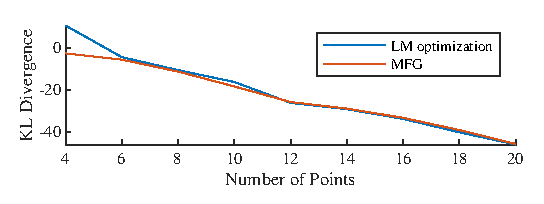
\includegraphics[scale=1.4]{figures/VIO-KL}
	\caption[KL divergence of the MFG and LM-optimization methods.]{KL divergence $d(p||p_\text{MFG})$ and $d(p||p_\text{LM})$ of the MFG and LM-optimization methods.}
	\label{fig:VIO-KL}
\end{figure}

The results are presented in Figure \ref{fig:VIO-KL}.
Because the constant $\log(c)$ is not calculated, the KL divergence in the figure is sometimes negative.
It can be seen that when $N>10$, the KL divergence for the LM method is slightly lower, indicating a slightly better estimation of the uncertainty.
When $N \leq 10$, because the uncertainty in pose increases, the KL-divergence of the MFG becomes smaller.
And when $N=4$ or 3, it becomes notably smaller than the LM method, indicating MFG is more accurate when dealing with very large uncertainty in the pose.

Next, the pose estimation algorithms is challenged with a singular configuration when the attitude has one degree of freedom that is not properly observed.
More specifically, the true attitude is set as $R_t = \expb{\tfrac{\pi}{2}\hat{e}_1}\expb{\tfrac{\pi}{2}\hat{e}_2}$, and the true translation is set as $t_t = [0,0,0]^T$.
There are ten map points, scattered as $p_i = [5,0,0]^T + \xi_i$, where $\xi_i\in\mathbb{R}^3$ is a three dimensional uniform distribution on $[-1,1] \times [-a,a]^2$, and $a$ is varied in $\{1,0.1,0.01,0\}$.
As $a$ is decreased, the map points are closer to the $e_1$-axis of the inertial frame, making the rotation about this axis gradually becomes unobservable.
The measurement noise is set as $A_1 = \cdots = A_N = 0.1^2I_{3\times 3}$.

\begin{table}
	\centering
	\caption{Estimation error $\pm$ S.D. ($p$-value) of the pose for a degenerative configuration}
	\label{tab:VIO-pose-error2}
	\footnotesize
	\begin{tabular}{l|cccc}
		\hline\hline
		estimator & \multicolumn{4}{c}{MFG} \\ \hline
		a & 1 & 0.1 & 0.01 & 0 \\ \hline
		att err (deg) & 3.93$\pm$1.79 (0.448) & 24.0$\pm$21.7 (0.642) & 82.4$\pm$51.4 (0.065) & 90.1$\pm$0.2 (0.279) \\
		pos err & 0.28$\pm$0.15 (0.339) & 0.36$\pm$0.20 (<0.001) & 0.14$\pm$0.06 (<0.001) & 0.11$\pm$0.08 (<0.001) \\
		\midrule[1.2pt]
		estimator & \multicolumn{4}{c}{LM optimization} \\ \hline
		a & 1 & 0.1 & 0.01 & 0 \\ \hline
		att err (deg) & 3.93$\pm$1.79 & 24.0$\pm$21.8 & 80.7$\pm$51.2 & 90.1$\pm$0.1 \\
		pos err & 0.28$\pm$0.15 & 0.39$\pm$0.22 & 0.39$\pm$0.22 & 0.38$\pm$0.20 \\
		\hline\hline
	\end{tabular}
\end{table}

The estimation errors of the MFG and LM methods are listed in Table \ref{tab:VIO-pose-error2}.
It is shown that the two methods have very similar accuracy of attitude errors, and the error becomes very large when $a = 0.01$ or 0, indicating that the attitude cannot be fully observed due to the placement of the map points.
On the other hand, the translation accuracy of the MFG method is much better than the LM optimization when $a = 0.01$ or 0.
Inspection of the Jacobian $J_r^TJ_R$ indicates that it becomes almost singular, due to the unobservability of attitude for the LM optimization.
Since $J_r^TJ_R$ is used to calculate the step size in the LM-optimization, this possibly explains why it has worse accuracy.
Interestingly, when $a$ is close to zero, the translation accuracy is even better than that when $a$ is relatively large.

Finally, the measurement update algorithm in Table \ref{tab:VIO-update} is combined with the uncertainty propagation in Table \ref{tab:posEst-prop} into a recursive Bayesian filter.
This filter is compared with the MEKF based method in a visual-inertial navigation setting.
A vehicle is supposed to move in a circle with radius of $\SI{3}{\meter}$.
The height of the trajectory is fluctuating between $\SI{0}{\meter}$ and $\SI{1}{\meter}$ as a sinusoidal function with the frequency at $\SI{0.785}{\hertz}$.
The resulting average free acceleration is $\SI{0.51}{\meter/\second\squared}$.
The first body-fixed axis of the vehicle points forward along the tangent direction of the trajectory, and the second body-fixed axis is confined in the horizontal plane, pointing towards the center of the circle.
The resulting average angular velocity is $\SI{24.7}{\deg/\second}$.
A hundred landmarks are scattered around the trajectory in a rectangular shape.
The trajectory of the vehicle and locations of landmarks are depicted in Figure \ref{fig:VIO-trajectory}.
A landmark is measured by the camera only if it is within $\SI{3}{\meter}$ of the vehicle.

\begin{figure}
	\centering
	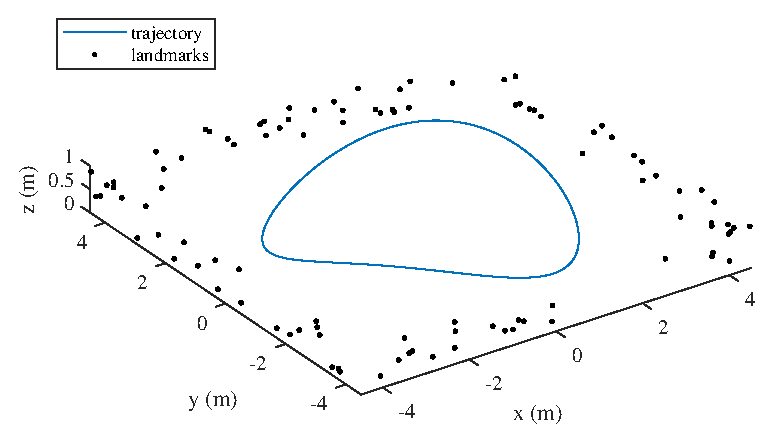
\includegraphics{figures/VIO-trajectory}
	\caption{Trajectory and landmarks for visual-inertial navigation.}
	\label{fig:VIO-trajectory}
\end{figure}

The white noise for the gyroscope is set as $\SI{0.1}{\deg/\sqrt{\second}}$, and for the accelerometer is $\SI{0.1}{\meter/\second/\sqrt{\second}}$.
It is assumed that the gyroscope and accelerometer do not have random walk biases, i.e., $H_{gv}$ in \eqref{eqn:posEst-kinematics-gyrobias} and $H_{av}$ in \eqref{eqn:posEst-kinematics-accebias} are zero, so the biases are not estimated in the filter.
The gyroscope is sampled at $\SI{200}{\hertz}$.
The position measurement noise of the camera is set identically as $\sigma^2I_{3\times 3}$, with $\sigma = \SI{1}{\meter}$.
And the sampling frequency for the camera is at $\SI{10}{\hertz}$.
The simulation lasts for $\SI{40}{\second}$.

Two initial conditions are tested.
For the first case, the initial attitude uncertainty for the MFG filter is $S_0 = 50I_{3\times 3}$, and for MEKF is $0.1^2I_{3\times 3}$.
The initial velocity and position uncertainties for both filters are set as $0.1^2I_{3\times 3}$.
The initial attitude, velocity, and position are their true values plus a random noise sampled from those initial uncertainty distributions.
This corresponds to an initial condition with relatively small uncertainty.
Next, for the second case, the initial conditions for velocity and position are set the same as in the first case.
But the initial attitude is rotated from the true attitude around the inertial vertical axis by $\SI{180}{\deg}$, simulating the scenario when the initial heading direction is completely unknown.
The attitude uncertainty for MFG is set as $S_0 = 0.01I_{3\times 3}$, and for MEKF is $1000I_{3\times 3}$, indicating a very large initial attitude uncertainty.
A hundred Monte Carlo simulations are carried out for both initial conditions, and paired $t$-test is used to find any significant difference with the significant level at $\alpha = 0.001$.

\begin{table}
	\centering
	\footnotesize
	\caption{Estimation error for visual-inertial navigation without map noises}
	\label{tab:VIO-filter-error}
	\begin{tabular}{l|c|c|c|c}
		\hline\hline
		initial condition & \multicolumn{2}{c|}{small uncertainty} & \multicolumn{2}{c}{large uncertainty} \\ \hline
		filter & MFG & MEKF & MFG & MEKF \\ \hline
		att err (deg) & 0.97$\pm$0.21 (p<0.001) & 0.90$\pm$0.20 & 1.62$\pm$0.23 (p<0.001) & 75.0$\pm$38.5 \\
		vel err (m/s) & 0.208$\pm$0.012 (p<0.001) & 0.205$\pm$0.013 & 0.235$\pm$0.013 (p<0.001) & 1.59$\pm$0.54 \\
		pos err (m) & 0.173$\pm$0.011 (p<0.001) & 0.172$\pm$0.011 & 0.184$\pm$0.010 (p<0.001) & 2.37$\pm$1.03 \\
		\hline\hline
	\end{tabular}
\end{table}

\begin{figure}
	\centering
	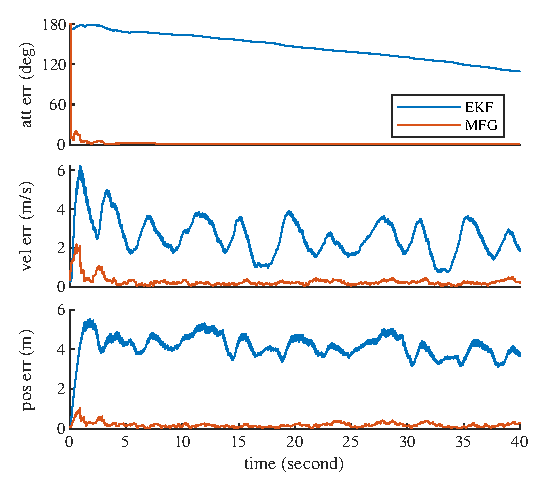
\includegraphics[scale=1.3]{figures/VIO-filter-error}
	\caption{Error trajectory of a particular simulation for visual-inertial navigation without map noises.}
	\label{fig:VIO-filter-error}
\end{figure}

For the MFG filter, only definition MFGI is tested, because all linear components, i.e., velocity and position, are defined in the inertial frame.
The estimation errors for MFG and MEKF are summarized in Table \ref{tab:VIO-filter-error}.
It demonstrates that MEKF has slightly better accuracy than MFG for the small initial uncertainty case, which is consistent with the results in Table \eqref{tab:VIO-pose-error} for static pose estimation.
But their relative differences are very small compared to the magnitude of error.
On the other hand, for large initial uncertainty, the MFG filter behaves much better than MEKF.
The trajectory of the estimation error for one particular simulation is presented in Figure \ref{fig:VIO-filter-error}.
It is seen that the MEKF suffers from extremely slow convergence from the initially wrong attitude.
Even worse, the wrong attitude estimation for MEKF contributes to the large errors in velocity and position.
This is very similar to the simulation for IMU-GNSS navigation in Figure \ref{fig:posEst-error}.
And the reason for this slow convergence can be attributed to that the Gaussian distribution of MEKF does not properly describe the initial large attitude uncertainty.

\subsection{Pose Estimation With Map Uncertainty} \label{section:VIO-pose-map}

In Chapter \ref{section:VIO-pose}, an algorithm is developed to model the uncertainty of the pose $(R,t)\in\SE{3}$ that aligns two point sets.
In particular, the map point set is assumed to be perfectly known, and the measurement point set is affected by random noises.
However, in some cases the noise of map point set also needs to be modeled.
For example, the 3D coordinates of triangulated features from a stereo camera have larger noises when the feature is further away from the camera, so it may be beneficial to also model the uncertainty of those triangulated map points.
In this subsection, the MFG is used to model the pose where the map point set also suffers from noises.

Suppose there are $N$ landmarks, whose coordinates in the inertial frame are denoted by $\{p_i\}_{i=1}^N$.
The coordinates are randomly distributed by $p_i \sim \mathcal{N}(\bar{p}_i, B_i)$.
These map points are measured by a camera in the body fixed frame as $\{p'_i\}_{i=1}^N$, affected by Gaussian noises with zero mean and covariance matrices $A_i = \sigma_i^2I_{3\times 3}$.
Note that only the noise of measurements $A_i$ is assumed to be isotropic.
If there is no prior information for the pose (non-informative prior), the posterior density function for the pose and map, according to the Bayes' formula, is given by
\begin{align} \label{eqn:VIO-likelihood-map}
	p\left( R,t,\{p_i\} | \{p'_i\} \right) &\propto \expb{-\tfrac{1}{2} \sum_{i=1}^{N} \big(R^T(p_i-t)-p'_i\big)^T A_i^{-1} \big(R^T(p_i-t)-p'_i\big)} \nonumber \\
	&\qquad\qquad \cdot \expb{-\tfrac{1}{2}\sum_{i=1}^N (p_i-\bar{p}_i)^T B_i^{-1} (p_i-\bar{p}_i)}.
\end{align}
The first exponential term in the above equation is the likelihood \eqref{eqn:VIO-likelihood} considered in Chapter \ref{section:VIO-pose}, and the last term is the prior density function for map points.
The objective is to model the pose $(R,t)|\{p'_i\}$ with an MFG, and to find the posterior Gaussian distribution for each map point $p_i|\{p'_i\}$.

Because the coordinates of map points $p_i$ are now random variables, the algorithm developed in Chapter \ref{section:VIO-pose} cannot be directly used.
But in the next lemma, it is shown that \eqref{eqn:VIO-likelihood-map} can be decomposed into two parts, and one of them has exactly the same structure as \eqref{eqn:VIO-likelihood}, so the algorithm in Chapter \ref{section:VIO-pose} can be applied.

\begin{lemma} \label{lemma:VIO-likelihood-map-factor}
	Let $\delta p_i = p_i-\bar{p}_i \in \mathbb{R}^3$ for $i=1,\dots,N$. Equation \eqref{eqn:VIO-likelihood-map} can be decomposed into
	\begin{align}
		p(R,t,\{p_i\}|\{p'_i\}) = p(R,t|\{p'_i\}) p(\{\delta p_i\}|R,t,\{p'_i\}),
	\end{align}
	where $p(R,t|\{p'_i\})$ is
	\begin{align} \label{eqn:VIO-likelihood-map-Rt}
		\expb{-\tfrac{1}{2} \sum_{i=1}^N \big(R^T(\bar{p}_i-t)-p'_i\big)^T (A_i+R^TB_iR)^{-1} \big(R^T(\bar{p}_i-t)-p'_i\big)}.
	\end{align}
	Let $K_i = (A_i^{-1}+B_i^{-1})^{-1} A_i^{-1} \in \mathbb{R}^{3\times 3}$, then $p(\{\delta p_i\}|R,t,\{p'_i\})$ is
	\begin{align} \label{eqn:VIO-likelihood-map-p}
		\expb{-\tfrac{1}{2} \sum_{i=1}^N \left( \delta p_i - K_i(Rp'_i+t-\bar{p}_i) \right)^T (A_i^{-1}+B_i^{-1}) \left( \delta p_i - K_i(Rp'_i+t-\bar{p}_i) \right)}.
	\end{align}
\end{lemma}
\begin{proof}
	Because $A_i = \sigma_i^2I_{3\times 3}$, for $R\in\SO{3}$, $RA_i^{-1}R^T = A_i^{-1}$.
	For $i=1,\ldots,N$, the exponent of \eqref{eqn:VIO-likelihood-map} can be written as
	\begin{align*}
		&\big(R^T(p_i-t)-p'_i\big)^T A_i^{-1} \big(R^T(p_i-t)-p'_i\big) + (p_i-\bar{p}_i)^T B_i^{-1} (p_i-\bar{p}_i) \\
		= &(\bar{p}_i+\delta p_i - t - Rp'_i)^T A_i^{-1} (\bar{p}_i+\delta p_i - t - Rp'_i) + \delta p_i^T B_i^{-1} \delta p_i \\
		= &(Rp'_i+t-\bar{p}_i)^T A_i^{-1} (Rp'_i+t-\bar{p}_i) - 2\delta p_i^T A_i^{-1} (Rp'_i+t-\bar{p}_i) + \delta p_i^T (A_i^{-1}+B_i^{-1}) \delta p_i.
	\end{align*}
	The last two terms can be further arranged into a quadratic form as
	\begin{align*}
		&\delta p_i^T (A_i^{-1}+B_i^{-1}) \delta p_i - 2\delta p_i^T A_i^{-1} (Rp'_i+t-\bar{p}_i) \\
		= &\left( \delta p_i - K_i(Rp'_i+t-\bar{p}_i) \right)^T (A_i^{-1}+B_i^{-1}) \left( \delta p_i - K_i(Rp'_i+t-\bar{p}_i) \right) \\
		&\qquad - (Rp'_i+t-\bar{p}_i)^T A_i^{-1} (A_i^{-1}+B_i^{-1})^{-1} A_i^{-1} (Rp'_i+t-\bar{p}_i).
	\end{align*}
	Using the Woodbury matrix identity \cite{petersen2008matrix}, $(Rp'_i+t-\bar{p}_i)^T A_i^{-1} (Rp'_i+t-\bar{p}_i)$ and the last term in the above equation can be combined into
	\begin{align*}
		&(Rp'_i+t-\bar{p}_i)^T A_i^{-1} (Rp'_i+t-\bar{p}_i) - (Rp'_i+t-\bar{p}_i)^T A_i^{-1} (A_i^{-1}+B_i^{-1})^{-1} A_i^{-1} (Rp'_i+t-\bar{p}_i) \\
		&\qquad = (Rp'_i+t-\bar{p}_i)^T \Big[ A_i^{-1} - A_i^{-1} (A_i^{-1}+B_i^{-1})^{-1} A_i^{-1} \Big] (Rp'_i+t-\bar{p}_i) \\
		&\qquad = (Rp'_i+t-\bar{p}_i)^T (A_i+B_i)^{-1} (Rp'_i+t-\bar{p}_i) \\
		&\qquad = \big(R^T(\bar{p}_i-t)-p'_i\big)^T (A_i+R^TB_iR)^{-1} \big(R^T(\bar{p}_i-t)-p'_i\big).
	\end{align*}
	And the desired decomposition is derived.
\end{proof}

The density $p(R,t|\{p'_i\})$ in \eqref{eqn:VIO-likelihood-map-Rt} has exactly the same structure as \eqref{eqn:VIO-likelihood}, except the noise is increased from $A_i$ to $A_i+R^TB_iR$.
So using Theorem \ref{thm:VIO-factor} and \eqref{eqn:VIO-likelihood-marginal-q}, $p(R,t|\{p'_i\})$ can be further decomposed into
\begin{align} \label{eqn:VIO-likelihood-map-Rt-factor}
	&p(R,t|\{p'_i\}) = \expb{-\tfrac{1}{2} (\bm{q}'-\bm{q}_m)^T \big(\mathbf{T}\mathbf{A}\mathbf{T}^T\big)^{-1} (\bm{q}'-\bm{q}_m)} \nonumber \\
	&\qquad \cdot \expb{-\tfrac{1}{2} (t - \mu_{t|R})^T (RCR^T)^{-1} (t - \mu_{t|R})} \triangleq p(R|\{p'_i\}) p(t|R,\{p'_i\}),
\end{align}
where $\bm{q}'$ and $\bm{q}_m$ are defined in \eqref{eqn:VIO-centering}, with $p_i$ replaced by $\bar{p}_i$.
The covariance matrix $\mathbf{A} = \diag(A_1+RB_1R^T, \ldots, A_N+RB_NR^T)$, and $\mathbf{T}$, $\mu_{t|R}$ are defined in Theorem \ref{thm:VIO-factor}.
The first exponential term $p(R|\{p'_i\})$ can be matched to a matrix Fisher density using the algorithm in Table \ref{tab:VIO-marginal}, with $A_i$ replaced by $A_i+B_i$.
Note that although the definition of $\mathbf{A}$ has $RB_iR^T$, it can be simply replaced by $B_i$ in the proposal distribution for importance sampling, as the proposal distribution only needs to be close to the target distribution.

Let the approximated parameter of the matrix Fisher distribution be denoted by $F$.
And let $F = USV^T$ be its pSVD, define $\nu_R = (QS-SQ^T)^\vee$ for MFGI, or $\nu_R = (SQ-Q^TS)^\vee$ for MFGB, with $Q = U^TRV$ as before.
The next step is to study the density function
\begin{align*}
	p(t|R,\{p'_i\}) p(\{\delta p_i\}|R,t,\{p'_i\})
\end{align*}
conditioned by $R$.
The next lemma deals with this density.

\begin{lemma} \label{lemma:VIO-likelihood-tp}
	Let $\bm{x} = \left[p_1^T, \cdots, p_N^T, t^T\right]^T \in \mathbb{R}^{3N+3}$, and $\bm{\mu}_{x|R} = \left[\mu_{p_1|R}^T, \cdots, \mu_{p_N|R}^T, \mu_{t|R}^T\right]^T \in \mathbb{R}^{3N+3}$, where $\mu_{p_i|R} = (I_{3\times 3}-K_i)\bar{p}_i + K_i(Rp'_i+\mu_{t|R})$.
	Also, let $\bm{\Sigma}_{x|R}$ be defined as
	\begin{align} \label{eqn:VIO-likelihood-map-Sigmax}
		\bm{\Sigma}_{x|R} = \begin{bmatrix}
			A_1^{-1}+B_1^{-1} & \cdots & 0_{3\times 3} & -A_1^{-1} \\
			\vdots & \ddots & \vdots & \vdots \\
			0_{3\times 3} & \cdots & A_N^{-1}+B_N^{-1} & -A_N^{-1} \\
			-A_1^{-1} & \cdots & -A_N^{-1} & (RCR^T)^{-1} + \sum_{i=1}^N A_i^{-1}\left( A_i^{-1}+B_i^{-1} \right)^{-1} A_i^{-1}
		\end{bmatrix}^{-1}.
	\end{align}
	Then the conditional density can be written as
	\begin{align} \label{eqn:VIO-likelihood-map-tp}
		p(t|R,\{p'_i\}) p(\{\delta p_i\}|R,t,\{p'_i\}) = \expb{-\tfrac{1}{2} (\bm{x}-\bm{\mu}_{x|R})^T \bm{\Sigma}_{x|R}^{-1} (\bm{x}-\bm{\mu}_{x|R})}.
	\end{align}
\end{lemma}
\begin{proof}
	The mean of $\delta p_i$ in \eqref{eqn:VIO-likelihood-map-p} can be arranged into
	\begin{align*}
		K_i(Rp'_i+t-\bar{p}_i) = K_i(Rp'_i+\mu_{t|R}-\bar{p}_i) + K_i(t-\mu_{t|R}).
	\end{align*}
	Let $\mu_{\delta p_i|R} = K_i(Rp'_i+\mu_{t|R}-\bar{p}_i)$, then the exponent of $p(\{\delta p_i\}|R,t,\{p'_i\})$ becomes
	\begin{align*}
		&\left( \delta p_i - K_i(Rp'_i+t-\bar{p}_i) \right)^T (A_i^{-1}+B_i^{-1}) \left( \delta p_i - K_i(Rp'_i+t-\bar{p}_i) \right) \\
		= &\left( \begin{bmatrix} I_{3\times 3} & -K_i \end{bmatrix} \begin{bmatrix} \delta p_i - \mu_{\delta p_i|R} \\ t-\mu_{t|R} \end{bmatrix} \right)^T (A_i^{-1} + B_i^{-1}) \left( \begin{bmatrix} I_{3\times 3} & -K_i \end{bmatrix} \begin{bmatrix} \delta p_i - \mu_{\delta p_i|R} \\ t-\mu_{t|R} \end{bmatrix} \right) \\
		= &\begin{bmatrix} p_i - \mu_{p_i|R} \\ t-\mu_{t|R} \end{bmatrix}^T \begin{bmatrix} A_i^{-1} + B_i^{-1} & -A_i^{-1} \\ -A_i^{-1} & A_i^{-1}(A_i^{-1} + B_i^{-1})A_i^{-1} \end{bmatrix} \begin{bmatrix} p_i - \mu_{p_i|R} \\ t-\mu_{t|R} \end{bmatrix}.
	\end{align*}
	And \eqref{eqn:VIO-likelihood-map-tp} can be proved by summing up the above equations for $i=1,\ldots,N$, and $(t-\mu_{t|R})^T(RCR^T)^{-1}(t-\mu_{t|R})$.
\end{proof}

The conditional density for the map coordinates $\{p_i\}$ and translation $t$ is written into a Gaussian density in \eqref{eqn:VIO-likelihood-map-tp}, with the mean and variance dependent on $R$.
Because the objective is to match an MFG to $(R,t)|\{p'_i\}$, and Gaussian distributions to $p_i|\{p'_i\}$, only the covariance matrices for $t$ and each of $p_i$ are needed.
Namely, the diagonal blocks of $\Sigma_{x|R}$ in \eqref{eqn:VIO-likelihood-map-Sigmax} need to be evaluated, whereas the off-diagonal blocks representing correlations are neglected.
Using the block inversion formula, the $i$-th 3-by-3 diagonal block of $\bm{\Sigma}_{x|R}$ representing the conditional covariance matrix for $p_i$ is
\begin{align}
	\Sigma_{p_i|R} = B_i - B_i \left[ (A_i+B_i)^{-1} (A_i+B_i - RCR^T) (A_i+B_i)^{-1} \right] B_i.
\end{align}
And the last 3-by-3 diagonal block of $\bm{\Sigma}_{x|R}$ representing the conditional covariance matrix for $t$ is
\begin{align}
	\Sigma_{t|R} = RCR^T.
\end{align}
In other words, when matching $(R,t)|\{p'_i\}$ to an MFG, the map coordinates $\{p_i\}$ are marginalized; and when matching $p_i|\{p'_i\}$ to a Gaussian distribution, the pose $(R,t)$ and all other $\{p_j\}$ with $i\neq j$ are marginalized.

Before giving necessary moments for the conditional MLE of $t|R$, and the first two moments for $p_i$, note that the expressions of $C$ and $\mathbf{D}$ in \eqref{eqn:VIO-likelihood-C} and $\eqref{eqn:VIO-likelihood-D}$ are now defined using $\mathbf{A} = \diag(A_1+RB_1R^T, \ldots, A_N+RB_NR^T)$ in \eqref{eqn:VIO-likelihood-map-Rt} in this subsection.
So a similar lemma as Lemma \ref{lemma:VIO-likelihood-CD} is needed to simplify calculations.

\begin{lemma}
	Define $\tilde{C} = RCR^T \in \mathbb{R}^{3\times 3}$, and $\tilde{\mathbf{D}} \in \mathbb{R}^{3\times 3N}$ such that the $i$-th 3-by-3 column block of $\tilde{\mathbf{D}}$ is $\tilde{D}_i = RD_iR^T$.
	If the expressions of $C$ and $\mathbf{D}$ in \eqref{eqn:VIO-likelihood-C} and $\eqref{eqn:VIO-likelihood-D}$ are defined using $\mathbf{A} = \diag(A_1+RB_1R^T, \ldots, A_N+RB_NR^T)$, then $\tilde{C}$ and $\tilde{\mathbf{D}}$ have the same expressions as $C$ and $\mathbf{D}$ with $\mathbf{A} = \diag(A_1+B_1,\ldots,A_N+B_N)$.
\end{lemma}
\begin{proof}
	This lemma is a straightforward extension of Lemma \ref{lemma:VIO-likelihood-CD}.
\end{proof}

With the above lemma, the expressions for $\tilde{C}$ and $\tilde{\mathbf{D}}$ do not dependent on $R$ anymore.
Also, the conditional mean $\mu_{t|R}$ is simplified as follows
\begin{align}
	\mu_{t|R} = \sum_{i=1}^N \tilde{D}_i(Rp'_i-\bar{p}_i).
\end{align}
With these simplifications, the conditional mean $\mu_{t|R}$ and covariance matrices $\Sigma_{x|R}$ has exactly the same expression as in \eqref{eqn:VIO-likelihood-conditional-sim}, so the moments $\expect{t}$, $\expect{t\nu_R^T}$, and $\expect{tt^T}$ according to \eqref{eqn:VIO-likelihood-map-tp}, that are necessary for the conditional MLE, can be calculated as in Theorem \ref{thm:VIO-conditional} or Theorem \ref{thm:VIO-conditional-sim}, with $C$, $D_i$, and $p_i$ replaced by $\tilde{C}$, $\tilde{D}_i$, and $\bar{p}_i$, depending on whether $A_1+B_1 = \cdots = A_N+B_N$.
Also, the moments $\expect{p_i}$ and $\expect{p_ip_i^T}$ are given as follows.

\begin{theorem} \label{thm:VIO-likelihood-Ep}
	The moments $\expect{p_i}$ and $\expect{p_ip_i^T}$ according to \eqref{eqn:VIO-likelihood-map-tp} can be calculated as
	\begin{align}
		\expect{p_i} &= (I_{3\times 3}-K_i)\bar{p}_i + K_i(\expect{R}p'_i+\expect{\mu_{t|R}}), \\
		\expect{p_ip_i^T} &= \Sigma_{p_i|R} + (I_{3\times 3}-K_i)\bar{p}_i\bar{p}_i^T(I_{3\times 3}-K_i)^T + (I_{3\times 3}-K_i)\bar{p}_i (\expect{R}p'_i+\expect{\mu_{t|R}})^TK_i^T \nonumber \\
		&\quad + K_i \left(\expect{Rp'_i(p'_i)^TR^T} + \expect{Rp'_i\mu_{t|R}^T} + \expect{\mu_{t|R}(p'_i)^TR^T} + \expect{\mu_{t|R}\mu_{t|R}^T}\right) K_i^T \nonumber \\
		&\quad + K_i(\expect{R}p'_i+\expect{\mu_{t|R}})\bar{p}_i^T(I_{3\times 3}-K_i)^T,
	\end{align}
	where $\expect{\mu_{t|R}} = \expect{t}$, $\expect{\mu_{t|R}\mu_{t|R}^T} = \expect{tt^T} - \tilde{C}$.
	Also, if $A_1+B_1 = \cdots = A_N+B_N$, then
	\begin{align}
		\expect{\mu_{t|R}(p'_i)^TR^T} = \bar{p}_c(p'_i)^T\expect{R}^T - \expect{Rp'_c(p'_i)^TR^T},
	\end{align}
	otherwise
	\begin{align}
		\expect{\mu_{t|R}(p'_i)^TR^T} = \sum_{j=1}^N \tilde{D}_j \left(\expect{Rp'_j(p'_i)^TR^T} - \bar{p}_j(p'_i)^T\expect{R}^T\right).
	\end{align}
\end{theorem}
\begin{proof}
	These moments can be calculated by integrating the left hand side with respect to the conditional density \eqref{eqn:VIO-likelihood-map-tp}, and noting that the marginal distribution of a multi-variate Gaussian distribution is also Gaussian with the corresponding mean and covariance matrix.
	Then the results are further integrated with respect to the marginal distribution for $R$, which has already been matched to a matrix Fisher distribution with parameter $F$.
\end{proof}

With the moments $\expect{p_i}$ and $\expect{p_ip_i^T}$, the distribution for $p_i$ can be matched to a Gaussian distribution with the same first and second order moments.
In summary, the posterior density \eqref{eqn:VIO-likelihood-map} has been approximated by an MFG for the pose $(R,t)$, and $N$ Gaussian distributions for the map coordinates $\{p_i\}_{i=1}^N$.
The pseudocode is summarized in Table \ref{tab:VIO-pose-map}.

\begin{table}
	\caption{Pose and map coordinates estimation with map noises}
	\label{tab:VIO-pose-map}
	\begin{algorithmic}[1]
		\algrule[0.8pt]
		\Procedure{($\mathcal{MG}, \{\mathcal{N}_i^+\}) = $ Pose-Map Estimation}{$\{p'_i\}$, $\{\mathcal{N}_i(\bar{p}_i,B_i)\}$}
		\algrule
		\State Obtain $F=$ Attitude Estimation($\{\bar{p}_i\}$, $\{p'_i\}$) in Table \ref{tab:VIO-marginal} with $A_i$ replaced by $A_i+B_i$, and $\expb{-\tfrac{1}{2}f_R(R)}$ as the first term on the right hand side of \eqref{eqn:VIO-likelihood-map-Rt-factor}.
		\State Let $F = USV^T$ be its pSVD.
		\State Calculate $\expect{\nu_R\nu_R^T}$ as in \eqref{eqn:MFG-EvRvR} using $S$.
		\If{$A_1+B_1 = \cdots = A_N+B_N$}
		\State Calculate $\expect{t}$, $\expect{t\nu_R^T}$, and $\expect{tt^T}$ in Theorem \ref{thm:VIO-conditional-sim}, with $\tfrac{\sigma^2}{N}I_{3\times 3}$ replaced by $\tfrac{A+B}{N}$, and $p_i$ replaced by $\bar{p}_i$.
		\Else
		\State Calculate $\expect{t}$, $\expect{t\nu_R^T}$, and $\expect{tt^T}$ in Theorem \ref{thm:VIO-conditional}, with $C$, $D_i$, and $p_i$ replaced by $\tilde{C}$, $\tilde{D}_i$, and $\bar{p}_i$.
		\EndIf
		\State Obtain $\mu$, $\Sigma$, $P$ according to Theorem \ref{thm:MFG-MLE-conditional}, with $\expect{t}$, $\expect{t\nu_R^T}$, $\expect{tt^T}$, $\expect{\nu_R\nu_R^T}$, and $\expect{\nu_R} = 0$.
		\State Set $\mathcal{MG} = \mathcal{MG}(\mu,\Sigma,P,U,S,V)$.
		\State For $i=1,\ldots,N$, calculate $\expect{p_i}$ and $\expect{p_ip_i^T}$ in Theorem \ref{thm:VIO-likelihood-Ep}.
		\State Set $\mathcal{N}_i^+$ as $\mathcal{N}(\expect{p_i}, \expect{p_ip_i^T}-\expect{p_i}\expect{p_i}^T)$.
		\EndProcedure
		\algrule[0.8pt]
	\end{algorithmic}
\end{table}

Next, then case when there is a prior density for the pose $(R,t)$ is also considered, so that the algorithm can be applied in a recursive filter.
Similar to Chapter \ref{section:VIO-pose}, let $y = [t^T, a^T]^T \in \mathbb{R}^n$, suppose $(R,y)$ follows an MFG with the parameter $(\mu,\Sigma,P,U,S,V)$ before measurements, where $a$ includes other Euclidean quantities, such as linear velocity and sensor biases.
According to the Bayes' formula, the posterior density for the pose $(R,y)$ and map coordinates $\{p_i\}$ after incorporating the measurements $\{p'_i\}$ is
\begin{align} \label{eqn:VIO-map-posterior}
	&p(R,y,\{p_i\}|\{p'_i\}) = \expb{-\tfrac{1}{2}\sum_{i=1}^N \big(R^T(p_i-Hy)-p'_i\big)^T A_i^{-1} \big(R^T(p_i-Hy)-p'_i\big)} \nonumber \\
	&\qquad \cdot \expb{-\tfrac{1}{2}\sum_{i=1}^N (p_i-\bar{p}_i)^T B_i^{-1} (p_i-\bar{p}_i)} \cdot \etr{FR^T} \expb{-\tfrac{1}{2}(y-\mu_c)^T \Sigma_c^{-1} (y-\mu_c)},
\end{align}
where $F$, $\mu_c$, $\Sigma_c$ are defined with respect to $\mathcal{MG}(\mu,\Sigma,P,U,S,V)$.
According to Lemma \ref{lemma:VIO-likelihood-map-factor}, Lemma \ref{lemma:VIO-likelihood-tp}, and \eqref{eqn:VIO-likelihood-map-Rt-factor}, the above density can be decomposed into
\begin{align} \label{eqn:VIO-map-posterior-factor1}
	&p(R,y,\{p_i\}|\{p'_i\}) = \etr{FR^T} \expb{-\tfrac{1}{2} (\bm{q}'-\bm{q}_m)^T \big(\mathbf{T}\mathbf{A}\mathbf{T}^T\big)^{-1} (\bm{q}'-\bm{q}_m)} \nonumber \\
	&\qquad \cdot \expb{-\tfrac{1}{2} (\bm{x}-\bm{\mu}_{x|R})^T \bm{\Sigma}_{x|R}^{-1} (\bm{x}-\bm{\mu}_{x|R})} \expb{-\tfrac{1}{2}(y-\mu_c)^T \Sigma_c^{-1} (y-\mu_c)}.
\end{align}
As before, this density function is factorized into a marginal density for $R$, and a conditional density for $t|R$, and $\{p_i\}|R$.

\begin{theorem} \label{thm:VIO-map-posterior}
	Let $z = [\bm{x}^T, a^T]^T \in \mathbb{R}^{3N+n}$, $H = \big[ I_{(3N+3)\times (3N+3)}, 0_{(3N+3)\times (n-3)} \big]$, and $G = \big[ 0_{n\times 3N}, I_{n\times n} \big]$.
	Define $\mu_{z|R}$ as
	\begin{align}
		\mu_{z|R} = \left( H^T\bm{\Sigma}_{x|R}^{-1}H + G^T\Sigma_c^{-1}G \right)^{-1} \left( H^T\bm{\Sigma}_{x|R}^{-1}\bm{\mu}_{x|R} + G^T\Sigma_c^{-1}\mu_c \right),
	\end{align}
	and $\Sigma_{z|R}$ as
	\begin{align}
		\Sigma_{z|R} = \left( H^T\bm{\Sigma}_{x|R}^{-1}H + G^T\Sigma_c^{-1}G \right)^{-1}.
	\end{align}
	Also, let $\mu_{c,t}$ and $\Sigma_{c,t}$ be the appropriate blocks in $\mu_c$ and $\Sigma_c$ for $t$.
	Then the posterior density $p(R,y,\{p_i\}|\{p'_i\})$ can be written as
	\begin{align} \label{eqn:VIO-map-posterior-factor2}
		&p(R,y,\{p_i\}|\{p'_i\}) = \etr{FR^T} \expb{-\tfrac{1}{2} (\bm{q}'-\bm{q}_m)^T \big(\mathbf{T}\mathbf{A}\mathbf{T}^T\big)^{-1} (\bm{q}'-\bm{q}_m)} \nonumber \\
		&\ \cdot \expb{-\tfrac{1}{2}(\mu_{t|R}-\mu_{c,t})^T (\Sigma_{t|R} + \Sigma_{c,t})^{-1} (\mu_{t|R}-\mu_{c,t})} \expb{-\tfrac{1}{2}(z-\mu_{z|R})^T \Sigma_{z|R}^{-1} (z-\mu_{z|R})}.
	\end{align}
\end{theorem}
\begin{proof}
	The proof is given in Appendix \ref{app:VIO-map-posterior}.
\end{proof}

The key point is that the first three terms on the right hand side of \eqref{eqn:VIO-map-posterior-factor2} do not depend on $z$, so they can be matched to a matrix Fisher distribution using the progressive update method in Table \ref{tab:posEst-update-att}.
As before, let the approximated parameter of the matrix Fisher distribution be denoted by $F^+$.
And let $F^+ = U^+S^+(V^+)^T$ be its pSVD, define $\nu_R = (Q^+S^+-S^+(Q^+)^T)^\vee$ for MFGI, or $\nu_R = (S^+Q^+-(Q^+)^TS^+)^\vee$ for MFGB, with $Q^+ = (U^+)^TR^+V^+$.
Similar to the case without pose prior, the next step is to calculate the moments for $y|R$ with $\{p_i\}$ marginalized out; and the moments for $p_i$, with $(R,y)$ and other $\{p_j\}$, $i\neq j$, marginalized out.
These moments are according to the posterior density \eqref{eqn:VIO-map-posterior-factor2}, and to distinguish with those according to the prior distribution $\mathcal{MG}(\mu,\Sigma,P,U,S,V)$, they are denoted by $\expect{\cdot | \mathcal{Z}}$, where $\mathcal{Z} = \{p'_i\}_{i=1}^N$ are all measurements.
The calculations for these moments are relegated to Theorem \ref{thm:VIO-map-posterior-moments} in Appendix \ref{app:VIO-map-posterior}.

Using the moments $\expect{y|\mathcal{Z}}$, $\expect{y(\nu_R^+)^T|\mathcal{Z}}$, and $\expect{yy^T|\mathcal{Z}}$, the posterior density for $(R,t)$ is matched to an MFG using the conditional MLE in Theorem \ref{thm:MFG-MLE-conditional}.
And using the moments $\expect{p_i|\mathcal{Z}}$ and $\expect{p_ip_i^T|\mathcal{Z}}$, the posterior density for $p_i$ is matched to a Gaussian distribution, for $i=1,\ldots,N$.
The pseudocode is summarized in Table \ref{tab:VIO-map-update}.

\begin{table}
	\caption{Measurement update with map noises}
	\label{tab:VIO-map-update}
	\begin{algorithmic}[1]
		\algrule[0.8pt]
		\Procedure{$(\mathcal{MG}^+,\{\mathcal{N}_i^+\})$ = Measurement Update}{$\mathcal{MG}^-$, $\{\mathcal{N}_i^-(\bar{p}_i,B_i)\}$, $\{p'_i\}$}
		\algrule
		\State Let $F^- = U^-S^-(V^-)^T$.
		\State Calculate $F^+=$ Attitude Update($F^-$, $\{\bar{p}_i\}$, $\{p'_i\}$) in Table \ref{tab:VIO-update}, where $f_m(R)$ is the second and third term on the right hand side of \eqref{eqn:VIO-map-posterior-factor2}.
		\State Let the pSVD of $F^+$ be $F^+ = U^+S^+(V^+)^T$.
		\State Calculate $\expect{y|\mathcal{Z}}$, $\expect{y(\nu_R^+)^T|\mathcal{Z}}$, and $\expect{yy^T|\mathcal{Z}}$ in Theorem \ref{thm:VIO-map-posterior-moments}.
		\State Obtain $\mu^+$, $\Sigma^+$, and $P^+$ using the conditional MLE in Theorem \ref{thm:MFG-MLE-conditional}.
		\State Set $\mathcal{MG}^+ = \mathcal{MG}(\mu^+,\Sigma^+,P^+,U^+,S^+,V^+)$.
		\State For $i=1,\ldots,N$, calculate $\expect{p_i|\mathcal{Z}}$ and $\expect{p_ip_i^T|\mathcal{Z}}$ in Theorem \ref{thm:VIO-map-posterior-moments}.
		\State Set $\mathcal{N}_i^+$ as $\mathcal{N}(\expect{p_i|\mathcal{Z}}, \expect{p_ip_i^T|\mathcal{Z}}-\expect{p_i|\mathcal{Z}}\expect{p_i|\mathcal{Z}}^T)$.
		\EndProcedure
		\algrule[0.8pt]
	\end{algorithmic}
\end{table}

\subsection{Numerical Simulations With Map Uncertainty}

The proposed method in the previous subsection that uses an MFG to model the pose that aligns two points set with noises is compared with an LM optimization method in this subsection.

First, the estimation algorithm in Table \ref{tab:VIO-pose-map} without pose prior is tested.
The true attitude is set as $R_t = \expb{\tfrac{\pi}{2}\hat{e}_3}$, and the true translation is $t_t = [5,0,0]^T$.
There are 10 map points, scattered as $\bar{p}_i = t_t + \xi_i$, where $\xi_i\in\mathbb{R}^3$ is a three dimensional uniform distribution on $[0,1]^3$.
The prior noise of $p_i$ are grouped into two levels, $N_1$ of them have small noise as $B_i = 0.1^2I_{3\times}$, and $10-N_1$ of them have large noise as $B_i = 1^2I_{3\times 3}$.
The measurement noise is set as $A_i = 0.1^2I_{3\times 3}$ for all $i=1,\ldots,10$.
The number $N_1$ is varied in $\{0,2,4,6,8,10\}$.
For each $N_1$, a thousand Monte Carlo simulations are carried out.
Paired $t$-tests are used to compare the attitude, translation, and map coordinate errors of the MFG algorithm and LM optimization.

\begin{table}
	\centering
	\caption{Pose and map coordinates errors with map uncertainty}
	\label{tab:VIO-error-pose-map}
	\footnotesize
	\begin{tabular}{l|ccc}
		\hline\hline
		estimator & \multicolumn{3}{c}{MFG} \\ \hline
		$N_1$ & 10 & 8 & 6 \\ \hline
		att err (deg) & 9.98$\pm$4.21 (p=0.061) & 10.7$\pm$4.9 (p=0.213) & 13.4$\pm$5.9 (p<0.001) \\
		pos err & 0.173$\pm$0.082 (p=0.240) & 0.198$\pm$0.098 (p=0.048) & 0.237$\pm$0.112 (p<0.001) \\
		map err ($N_1$) & 0.1237$\pm$0.0165 (p<0.001) & 0.126$\pm$0.020 (p<0.001) & 0.130$\pm$0.024 (p<0.001) \\
		map err ($10-N_1$) & - & 0.187$\pm$0.057 (p<0.001) & 0.205$\pm$0.050 (p<0.001) \\
		\midrule[1.2pt]
		estimator & \multicolumn{3}{c}{LM optimization} \\ \hline
		$N_1$ & 10 & 8 & 6 \\ \hline
		att err (deg) & 9.96$\pm$4.20 & 10.7$\pm$4.9 & 13.0$\pm$5.8 \\
		pos err & 0.174$\pm$0.083 & 0.197$\pm$0.099 & 0.230$\pm$0.113 \\
		map err ($N_1$) & 0.1241$\pm$0.0165 & 0.127$\pm$0.020 & 0.131$\pm$0.024 \\
		map err ($10-N_1$) & - & 0.191$\pm$0.058 & 0.209$\pm$0.050 \\
		\hline\hline
		estimator & \multicolumn{3}{c}{MFG} \\ \hline
		$N_1$ & 4 & 2 & 0 \\ \hline
		att err (deg) & 16.5$\pm$7.9 (p<0.001) & 50.6$\pm$30.9 (p<0.001) & 77.1$\pm$41.1 (p=0.056) \\
		pos err & 0.305$\pm$0.147 (p<0.001) & 0.755$\pm$0.372 (p=0.005) & 1.05$\pm$0.38 (p<0.001) \\
		map err ($N_1$) & 0.138$\pm$0.030 (p=0.033) & 0.149$\pm$0.046 (p<0.001) & - \\
		map err ($10-N_1$) & 0.225$\pm$0.056 (p<0.001) & 0.501$\pm$0.189 (p<0.001) & 0.661$\pm$0.173 (p<0.001) \\
		\midrule[1.2pt]
		estimator & \multicolumn{3}{c}{LM optimization} \\ \hline
		$N_1$ & 4 & 2 & 0 \\ \hline
		att err (deg) & 16.0$\pm$7.5 & 48.6$\pm$29.5 & 76.4$\pm$40.8 \\
		pos err & 0.294$\pm$0.149 & 0.772$\pm$0.455 & 1.17$\pm$0.55 \\
		map err ($N_1$) & 0.138$\pm$0.030 & 0.153$\pm$0.048 & - \\
		map err ($10-N_1$) & 0.230$\pm$0.056 & 0.518$\pm$0.216 & 0.708$\pm$0.196 \\
		\hline\hline
	\end{tabular}
\end{table}

The estimation errors are summarized in Table \ref{tab:VIO-error-pose-map}.
Generally speaking, the MFG algorithm has slightly worse accuracy in pose estimation, especially when $N_1 = 4$ and 6, indicating it may have degraded performance when the map prior has mixed uncertainty levels.
But when $N_1 = 0$, the translation error for MFG is significantly smaller than LM optimization, which is consistent with the results in Table \ref{tab:VIO-pose-error}.
Namely, when the pose has large uncertainty, the MFG is better at estimating the translation.
Next, looking at the map coordinate errors, in general the MFG algorithm is more accurate, especially for those points with large prior noises, where the differences are significant for all cases.
The reason for this better performance of MFG is to be investigated in future works, but a guess is that the gradient based optimization may not be very effective for high dimensional variable space, which is 66 in this simulation study; or that the parameters for the LM method is not properly tuned for this high dimensional space.

Next, the measurement update algorithm in Table \ref{tab:VIO-map-update} is combined with the uncertainty propagation for IMU in Table \ref{tab:posEst-prop} into a Bayesian filter for visual-inertial navigation.
And this filter is compared with an MEKF based SLAM algorithm which also estimates the map point coordinates.
In this simulation study, a vehicle is supposed to follow the same trajectory and rotational motion introduced in the simulation in Chapter \ref{section:VIO-simulation}.
The distribution of landmarks, noise parameters for the IMU, sampling frequencies for the IMU and camera are also chosen to be the same.
There are in total 400 landmarks, and the measurement noise of the camera is set as $A_i = 0.05^2I_{3\times 3}$.
Only the landmarks that are within $\SI{3}{\meter}$ from the vehicle are measured by the camera.
The simulation lasts for forty seconds.

Three cases are tested.
The first case is a \textit{normal} condition: the prior noise for all map coordinates are $B_i = 0.1^2I_{3\times 3}$.
The initial attitude, velocity, and position uncertainty for MEKF is set as $0.1^2I_{3\times 3}$; and the initial attitude uncertainty for MFG is $S_0 = 50I_{3\times 3}$.
The initial attitude, velocity, and position estimates are set as their true values plus random noises sampled from those initial uncertainty distributions.
Namely, the normal condition corresponds to small prior map noises, and initial conditions with relatively small uncertainty.
In the second case, the initial conditions are the same as the normal case, but the prior map noise is $B_i = 1^2I_{3\times 3}$, i.e., this corresponds to large map uncertainty.
In the third case, the map uncertainty is the same as the normal case.
But the initial attitude is rotated from the true attitude around the inertial vertical axis by $\SI{180}{\deg}$, simulating the scenario when the initial heading direction is completely unknown.
The initial attitude uncertainty for MFG is $S_0 = 0.01I_{3\times 3}$, and for MEKF is $1000I_{3\times 3}$.
One hundred Monte Carlo simulations are run for each of the three cases, and paired $t$-test ($\alpha=0.001$) is used to detect statistical significance.

\begin{table}
	\centering
	\caption{Estimation error for visual-inertial navigation with map noises}
	\label{tab:VIO-map-filter-error1}
	\small
	\begin{tabular}{l|cc}
		\hline\hline
		case & \multicolumn{2}{c}{normal} \\ \hline
		filter & MFG & MEKF \\ \hline
		att err (deg) & 0.65$\pm$0.25 (p<0.001) & 0.73$\pm$0.32 \\
		vel err (m/s) & 0.078$\pm$0.005 (p=0.004) & 0.079$\pm$0.005 \\
		pos err (m) & 0.042$\pm$0.015 (p<0.001) & 0.048$\pm$0.020 \\
		mean map err (m) & 0.044$\pm$0.014 (p<0.001) & 0.051$\pm$0.019 \\
		\hline\hline
		case & \multicolumn{2}{c}{large map uncertainty} \\ \hline
		filter & MFG & MEKF \\ \hline
		att err (deg) & 4.36$\pm$2.07 (p<0.001) & 5.12$\pm$2.08 \\
		vel err (m/s) & 0.158$\pm$0.054 (p<0.001) & 0.179$\pm$0.056 \\
		pos err (m) & 0.314$\pm$0.149 (p=0.006) & 0.355$\pm$0.152 \\
		mean map err (m) & 0.384$\pm$0.182 (p=0.002) & 0.441$\pm$0.185 \\
		\hline\hline
		case & \multicolumn{2}{c}{large initial uncertainty} \\ \hline
		filter & MFG & MEKF \\ \hline
		att err (deg) & 1.07$\pm$0.22 (p<0.001) & 101.64$\pm$ 0.23 \\
		vel err (m/s) & 0.082$\pm$0.004 (p<0.001) & 1.610$\pm$ 0.005 \\
		pos err (m) & 0.041$\pm$0.014 (p<0.001) & 5.033$\pm$0.014 \\
		mean map err (m) & 0.043$\pm$0.013 (p<0.001) & 6.167$\pm$0.010 \\
		\hline\hline
	\end{tabular}
\end{table}

The estimation results for the two filters are summarized in Table \ref{tab:VIO-map-filter-error1}.
For the first two cases, the MFG filter is slightly more accurate than MEKF, but their differences relative to the magnitude of errors are small.
This may be attributed to that the MFG filter has slightly better accuracy in map coordinate estimation as seen in Table \ref{tab:VIO-error-pose-map}, and the subsequent pose estimation relies on the map coordinates estimated in previous steps.
For the third case when the initial heading direction is completely reversed, the MFG filter performs much better than MEKF.
The estimation error for one particular simulation is presented in Figure \ref{fig:VIO-map-filter-error1}, and the estimated trajectory of the vehicle and final map point coordinates are shown in Figure \ref{fig:VIO-map-filter-trajectory1}.
Similar to the simulation without prior map noises (Figure \ref{fig:VIO-trajectory}), the MEKF suffers from convergence problems.
Moreover, since MEKF also estimates map coordinates in this simulation, they are also adversely affected by the wrong attitude estimation.
These large errors in the estimated map coordinates further contributes to large pose errors in the subsequent estimation, making the filter unable to converge at all.
Therefore, as seen in Figure \ref{fig:VIO-map-filter-error1}, the estimation error for MEKF becomes periodic as the vehicle circles around, i.e., it has smaller errors near where it starts because of the smaller map error.
This signifies the advantage of MFG filter that has very fast convergence speed thanks to its better accuracy when modeling large attitude uncertainty, and linearization free measurement update.

\begin{figure}
	\centering
	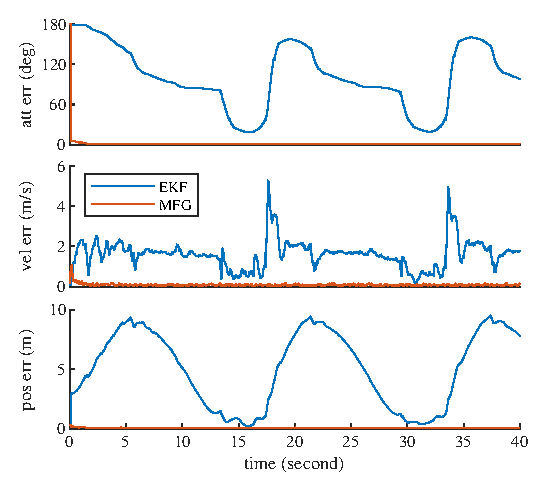
\includegraphics[scale=1.3]{figures/VIO-map-filter-error1}
	\caption{Estimation error of visual-inertial navigation with map noises.}
	\label{fig:VIO-map-filter-error1}
\end{figure}

\begin{figure}
	\centering
	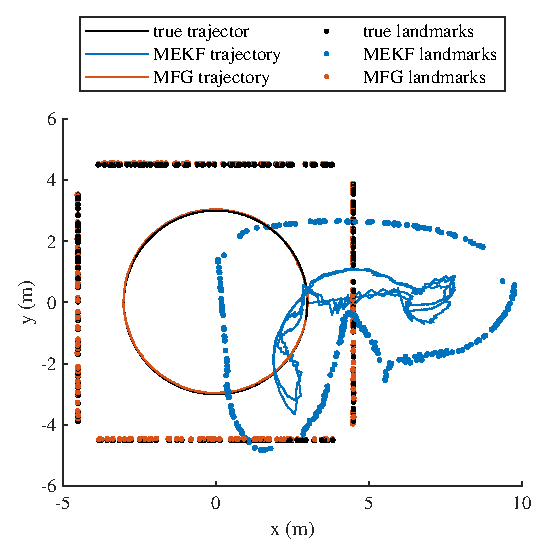
\includegraphics[scale=1.2]{figures/VIO-map-filter-trajectory1}
	\caption{Trajectory and landmarks of visual-inertial navigation with map noises.}
	\label{fig:VIO-map-filter-trajectory1}
\end{figure}

Finally, to test the proposed algorithm in visual-inertial odometry settings where there is no prior map information, the unknown map point is constructed using its measurement in the body-fixed frame by the camera.
More specifically, suppose the pose $(R,t)$ has a density function $p_{R,t}(R,t)$, and the map point $p_i$ is measured as $p'_i = R^T(p_i-t)$ in the body-fixed frame, with a density function $p_{p'_i}(p'_i)$.
Then using convolution, it can be shown that the probability density function of $p_i$ is
\begin{align} \label{eqn:VIO-transformPoint}
	p_{p_i}(p_i) = \int_{R\in\SO{3}} \int_{t\in\mathbb{R}^3} p_{R,t}(R,t) p_{p'_i}\left( R^T(p_i-t) \right) \diff t \diff R.
\end{align}
In particular, if $(R,t)$ follows an MFG, and $p'_i$ follows a Gaussian distribution, the density of $p_i$ becomes very complicated.
But its first and second order moments can be calculated as
\begin{align}
	\expect{p_i} &= \expect{R}p'_i + \expect{t} \\
	\expect{p_ip_i^T} &= \expect{Rp'_i(p'_i)^TR^T} + \expect{Rp'_it^T} + \expect{t(p'_i)^TR^T} + \expect{tt^T}.
\end{align}
So the distribution of $p_i$ can be matched to $\mathcal{N}(\expect{p_i}, \expect{p_ip_i^T}-\expect{p_i}\expect{p_i}^T)$.
But unfortunately, using Gaussian to model the distribution of $p_i$ is very inaccurate when $R$ has large uncertainty.
For example, if $R$ has a uniform distribution on $\SO{3}$, i.e., when $S = 0_{3\times 3}$, the density of $p_i$ is a spherical thin shell centered around $t$, which cannot be approximated by a Gaussian distribution.

As a consequence, for the third simulation case when the attitude error is initialized as $S = 0.01I_{3\times 3}$, the resulting uncertainty of the map coordinates cannot be accurately modeled by Gaussian.
In order to circumvent this problem but still test the proposed algorithm in visual-inertial odometry settings, in the next simulation, only the features measured in the first second are assumed to have a map prior, and subsequent map coordinates are modeled by Gaussian distribution with the first and second moments.

\begin{table}
	\centering
	\caption{Estimation error for visual-inertial odometry with map noises}
	\label{tab:VIO-map-filter-error2}
	\small
	\begin{tabular}{l|cc}
		\hline\hline
		case & \multicolumn{2}{c}{normal} \\ \hline
		filter & MFG & MEKF \\ \hline
		att err (deg) & 1.16$\pm$0.55 (p=0.066) & 1.25$\pm$0.66 \\
		vel err (m/s) & 0.086$\pm$0.012 (p=0.054) & 0.088$\pm$0.016 \\
		pos err (m) & 0.103$\pm$0.055 (p=0.310) & 0.108$\pm$0.063 \\
		mean map err (m) & 0.109$\pm$0.054 (p=0.221) & 0.115$\pm$0.061 \\
		\hline\hline
		case & \multicolumn{2}{c}{large map uncertainty} \\ \hline
		filter & MFG & MEKF \\ \hline
		att err (deg) & 4.47$\pm$2.07 (p<0.001) & 5.18$\pm$2.07 \\
		vel err (m/s) & 0.161$\pm$0.054 (p<0.001) & 0.180$\pm$0.056 \\
		pos err (m) & 0.321$\pm$0.150 (p=0.009) & 0.360$\pm$0.150 \\
		mean map err (m) & 0.393$\pm$0.183 (p=0.003) & 0.448$\pm$0.184 \\
		\hline\hline
		case & \multicolumn{2}{c}{large initial uncertainty} \\ \hline
		filter & MFG & MEKF \\ \hline
		att err (deg) & 1.56$\pm$0.55 (p<0.001) & 179.0$\pm$0.24 \\
		vel err (m/s) & 0.090$\pm$0.013 (p<0.001) & 2.328$\pm$0.005 \\
		pos err (m) & 0.098$\pm$0.056 (p<0.001) & 9.958$\pm$0.019 \\
		mean map err (m) & 0.104$\pm$0.053 (p<0.001) & 11.55$\pm$0.015 \\
		\hline\hline
	\end{tabular}
\end{table}

The estimation errors for the three cases are summarized in Table \ref{tab:VIO-map-filter-error2}.
For the normal, and large map uncertainty cases, the MFG filter is slightly more accurate than MEKF, but most differences are statistically insignificant, indicating that the MFG and Gaussian distributions work similarly well for these cases when then attitude uncertainty is relatively small.
However, when coming to the third case where the initial attitude uncertainty is very large, the MEKF again does not converge.
This is indicated in Figure \ref{fig:VIO-map-filter-error2}, where the estimation errors for a particular simulation is presented; and in Figure \ref{fig:VIO-map-filter-trajectory2}, where the trajectory of the vehicle and the estimated feature positions are shown.
In this simulation, because there are no map priors for the features measured after one second, the trajectory and map coordinates estimated by MEKF are exactly rotated around the vertical axis by $\SI{180}{\deg}$, i.e., they are not constrained by the map priors as in Figure \ref{fig:VIO-map-filter-trajectory1}.
This is usually considered to be successful in visual-inertial odometry algorithms since the shape of the trajectory is accurately estimated.
On the other hand, for the MFG filter, because the attitude successfully converges within one second when the map priors are available for the measured features, the subsequent trajectory and map coordinates follow around their respective true values.

\begin{figure}
	\centering
	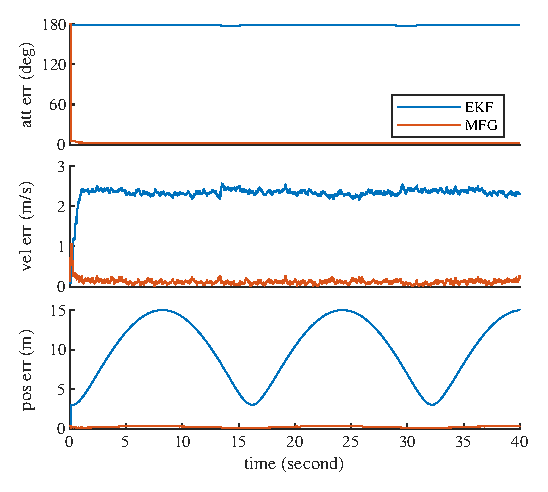
\includegraphics[scale=1.3]{figures/VIO-map-filter-error2}
	\caption{Estimation error of visual-inertial odometry with map noises.}
	\label{fig:VIO-map-filter-error2}
\end{figure}

\begin{figure}
	\centering
	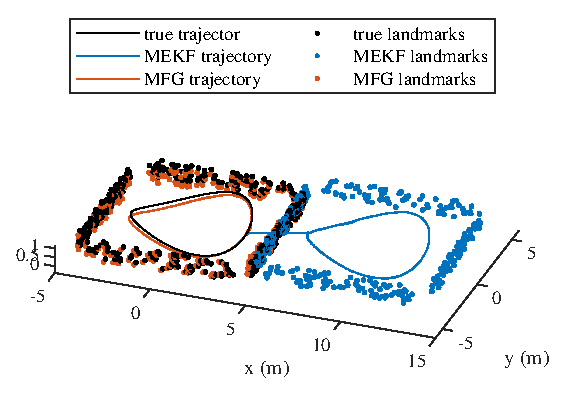
\includegraphics[scale=1.2]{figures/VIO-map-filter-trajectory2}
	\caption{Trajectory and features of visual-inertial odometry with map noises.}
	\label{fig:VIO-map-filter-trajectory2}
\end{figure}

As a summary, the MFG filter when applied to visual-inertial navigation or odometry problems, has similar accuracy with MEKF based algorithms when the initial attitude uncertainty is small.
Nevertheless, if the initial attitude uncertainty is very large, for example when the heading direction is completely unknown, the MFG filter has a much faster convergence rate from a wrong initial heading direction.

\subsection{Applications to the VCU-RVI Dataset}

The algorithms proposed in Chapter \ref{section:VIO-pose} and Chapter \ref{section:VIO-pose-map} are also tested with a real world IMU-RGBD dataset for visual-inertial odometry performance.
The VCU\_RVI dataset is used \cite{zhang2020vcu}, which is the only available dataset that has synchronized IMU and RGB-D camera measurements, together with ground truth from a motion capture system.
The data are collected with a BMI1055 IMU at $\SI{100}{\hertz}$, and a Structure Core RGB-D camera that provides the 3D coordinates of captured features in the camera's body-fixed frame at $\SI{30}{\hertz}$.
The five trials ``lab\_bumper1'' to ``lab\_bumper5'' are used, where the IMU and camera are attached to a wheeled robot, moving around an indoor environment installed with speed bumps to provide 3D motions.

Next, some implementation details of the algorithms are described.
The map is composed of a set of previously detected points, including their coordinates in the inertial frame (and their uncertainties for the algorithm in Chapter \ref{section:VIO-pose-map}), their ORB features \cite{mur2015orb}, their viewing directions (a unit vector connecting the camera and the position of the point in inertial frame), and time indices denoting the last frame in which they are detected.
The visual features are detected using the MATLAB \texttt{detectORBFeatures} function, and extracted into ORB features.
After valid points are detected for the current frame, they are matched
to the map.
Before matching, the search range is refined to those map points satisfying both the following two conditions:
(i) the distance from the camera to the point is between $\SI{0.5}{\meter}$ and $\SI{5}{\meter}$; (ii) the difference of viewing directions is within
$\SI{60}{\deg}$.
The distance and viewing directions are calculated using the predicted position of the camera using IMU.
Then, the ORB features from the current frame, and the ORB features from the reduced map are matched using the MATLAB \texttt{matchFeatures} function, with the \texttt{unique} parameter set as true, which means no feature will be matched with more than one features.
RANSAC is then applied to reduce mismatches.
The captured points that have been successfully matched to the map are used as the measurements in the current frame to correct the pose, and the map coordinates if the algorithm in Chapter \ref{section:VIO-pose-map} is used.

After matching, all valid points detected in the current frame, which are not matched to any point in the map, are transformed into the inertial frame using the estimated pose, and are added to the map.
Also, for the map points which are matched to the map in the current frame, their time indices are renewed to be the index of the current frame.
Then, all map points with time indices more than 10 frames older than the current frame, are deleted from the map.
In other words, loop closure is not considered in this test.

The algorithm proposed in Chapter \ref{section:VIO-pose}, where the map coordinates are fixed without any uncertainty, is denoted by ``MFGd'', and the corresponding MEKF is denoted by ``MEKFd''.
The algorithm in Chapter \ref{section:VIO-pose-map}, where the map coordinates are random variables with uncertainties, is denoted by ``MFGr'', and the corresponding MEKF is denoted by ``MEKFr''.
The definition MFGI is used in the MFG filters.
The white noise for the gyroscope is set as $\SI{0.1}{\deg/\sqrt{\second}}$, and for the accelerometer is $\SI{0.1}{\meter/\second/\sqrt{\second}}$.
It is assumed that the gyroscope and accelerometer have zero biases, so the bias is not estimated in the filter.
The noise for the camera measurements is set as $A_i = 0.002^2I_{3\times 3}$.
The attitude, velocity, and position of the robot is initialized as true values, and the initial uncertainties for them are set as $0.1^2I_{3\times 3}$.

The estimation results for the five trials: ``lab\_bumper1'' to ``lab\_bumper5'' are presented in Figure \ref{fig:VIO-dataset1} to Figure \ref{fig:VIO-dataset5}, and the final estimation errors are listed in Table \ref{tab:VIO-VCU_RVI}. 
It is seen that the tested four filtering algorithms have very similar estimation accuracy for the tested five trials.
In particular, the algorithms with map uncertainty behave better in the first and fifth trials, while worse in the other three, than the algorithms with fixed map coordinates.
The performance of the MFG filter and MEKF when the map is fixed is almost indistinguishable; whereas if the map coordinates have uncertainty, the MFG filter seems to be a little worse than MEKF.

As discussed in Chapter \ref{section:VIO-pose-map}, the uncertainty of map coordinates cannot be modeled by Gaussian distributions when the attitude uncertainty is large.
Therefore, for this odometry problem, the tested algorithms, including the MFG filters, cannot deal with wrong initial attitude as in the simulation studies.
Also, this testing with real world dataset is still too preliminary to draw any conclusions, as the parameters for the filters are not well tuned, and the sensor biases are not estimated.
These will be pursued in future works.

\begin{table}
	\centering
	\caption{Estimation errors for the VCU\_RVI dataset}
	\label{tab:VIO-VCU_RVI}
	\begin{tabular}{l|l|cccc}
		\hline\hline
		trials & & MFKFd & MFGd & MEKFr & MFGr \\ \hline
		\multirow{2}{*}{lab\_bumper1} & att err (deg) & 9.89 & 9.75 & 9.16 & 8.53 \\
		& pos err (m) & 0.399 & 0.395 & 0.264 & 0.281 \\ \hline
		\multirow{2}{*}{lab\_bumper2} & att err (deg) & 3.33 & 2.73 & 4.05 & 6.09 \\
		& pos err (m) & 0.069 & 0.095 & 0.069 & 0.076 \\ \hline
		\multirow{2}{*}{lab\_bumper3} & att err (deg) & 9.41 & 9.41 & 10.55 & 13.37 \\
		& pos err (m) & 0.676 & 0.677 & 0.672 & 0.738 \\ \hline
		\multirow{2}{*}{lab\_bumper4} & att err (deg) & 10.26 & 10.22 & 13.40 & 18.38 \\
		& pos err (m) & 0.919 & 0.863 & 0.975 & 0.984 \\ \hline
		\multirow{2}{*}{lab\_bumper5} & att err (deg) & 7.95 & 8.68 & 6.21 & 6.47 \\
		& pos err (m) & 0.635 & 0.663 & 0.610 & 0.561 \\
		\hline\hline
	\end{tabular}
\end{table}

\begin{figure}
	\centering
	\begin{subfigure}{\textwidth}
		\centering
		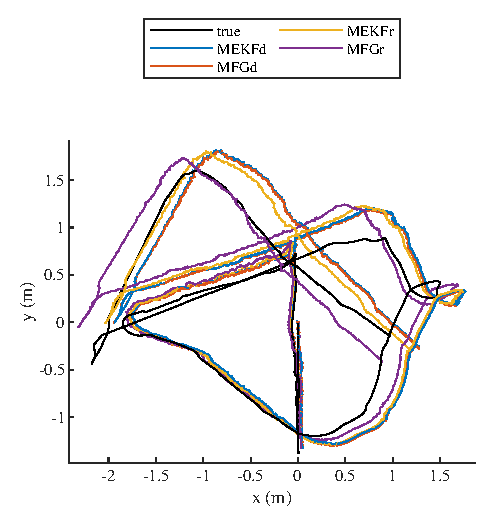
\includegraphics[scale=1.3]{figures/VIO-VCU_RVI-trajectory1}
	\end{subfigure}
	\begin{subfigure}{\textwidth}
		\centering
		\vspace{1cm}
		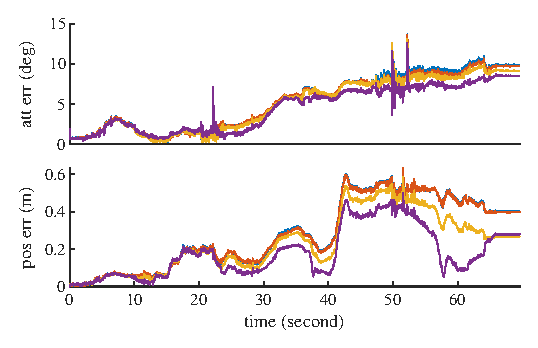
\includegraphics[scale=1.3]{figures/VIO-VCU_RVI-error1}
	\end{subfigure}
	\caption[Estimation errors for the ``lab\_bumper1'' trial.]{Estimation errors for the ``lab\_bumper1'' trial. The top row is the true and estimated trajectories.}
	\label{fig:VIO-dataset1}
\end{figure}

\begin{figure}
	\centering
	\begin{subfigure}{\textwidth}
		\centering
		\includegraphics[scale=1.3]{figures/VIO-VCU_RVI-trajectory2}
	\end{subfigure}
	\begin{subfigure}{\textwidth}
		\centering
		\vspace{1cm}
		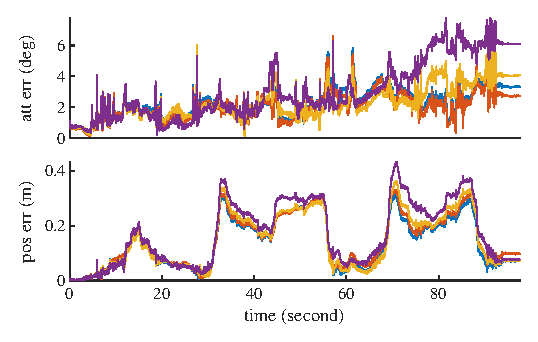
\includegraphics[scale=1.3]{figures/VIO-VCU_RVI-error2}
	\end{subfigure}
	\caption[Estimation errors for the ``lab\_bumper2'' trial.]{Estimation errors for the ``lab\_bumper2'' trial. The top row is the true and estimated trajectories.}
	\label{fig:VIO-dataset2}
\end{figure}

\begin{figure}
	\centering
	\begin{subfigure}{\textwidth}
		\centering
		\includegraphics[scale=1.3]{figures/VIO-VCU_RVI-trajectory3}
	\end{subfigure}
	\begin{subfigure}{\textwidth}
		\centering
		\vspace{1cm}
		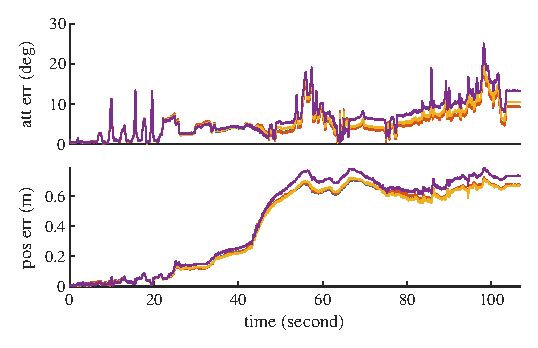
\includegraphics[scale=1.3]{figures/VIO-VCU_RVI-error3}
	\end{subfigure}
	\caption[Estimation errors for the ``lab\_bumper3'' trial.]{Estimation errors for the ``lab\_bumper3'' trial. The top row is the true and estimated trajectories.}
	\label{fig:VIO-dataset3}
\end{figure}

\begin{figure}
	\centering
	\begin{subfigure}{\textwidth}
		\centering
		\includegraphics[scale=1.3]{figures/VIO-VCU_RVI-trajectory4}
	\end{subfigure}
	\begin{subfigure}{\textwidth}
		\centering
		\vspace{1cm}
		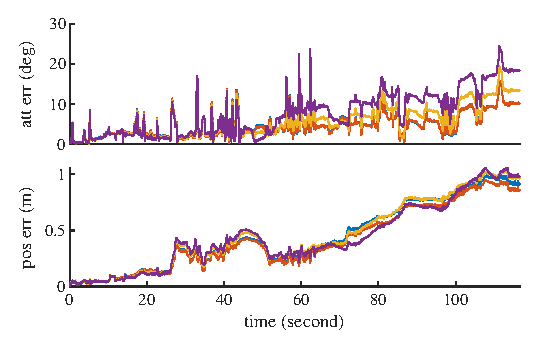
\includegraphics[scale=1.3]{figures/VIO-VCU_RVI-error4}
	\end{subfigure}
	\caption[Estimation errors for the ``lab\_bumper4'' trial.]{Estimation errors for the ``lab\_bumper4'' trial. The top row is the true and estimated trajectories.}
	\label{fig:VIO-dataset4}
\end{figure}

\begin{figure}
	\centering
	\begin{subfigure}{\textwidth}
		\centering
		\includegraphics[scale=1.3]{figures/VIO-VCU_RVI-trajectory5}
	\end{subfigure}
	\begin{subfigure}{\textwidth}
		\centering
		\vspace{1cm}
		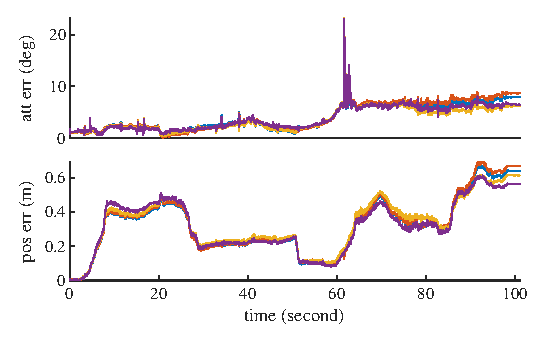
\includegraphics[scale=1.3]{figures/VIO-VCU_RVI-error5}
	\end{subfigure}
	\caption[Estimation errors for the ``lab\_bumper5'' trial.]{Estimation errors for the ``lab\_bumper5'' trial. The top row is the true and estimated trajectories.}
	\label{fig:VIO-dataset5}
\end{figure}
